\section{Synthetic Experiments}
\label{sec:expds}
We considered sparsity based simulations with varying $G$ and sparsity levels. In our first set of simulations, we set $p=100$, $G=10$ and sparsity of the individual parameters to be $s=10$. We generated a dense $\bbeta_0$ with $\|\bbeta_0\|=p$ and did not impose any constraint. Iterates $\{\bbeta^{(t)}_g\}_{g=1}^G$ are obtained by projection onto the $\ell_1$ ball $\|\bbeta_g\|_1$. Nonzero entries of $\bbeta_g$ are generated with ${\cal{N}}(0,1)$ and nonzero supports are picked uniformly at random. Inspired from our theoretical step size choices, in all experiments, we used simplified learning rates of $\frac{1}{n}$ for $\bbeta_0$ and $\frac{1}{\sqrt{nn_g}}$ for $\bbeta_g$, $g \in [G]_\setminus$. Observe that, cones of the individual parameters intersect with that of $\bbeta_0$ hence this setup actually violates DERIC (which requires an arbitrarily small constant fraction of groups to be non-intersecting). Our intuition is that the individual parameters are mostly incoherent with each other and the existence of a nonzero perturbation over $\bbeta_g$'s that keeps all measurements intact is unlikely. Remarkably, experimental results still show successful learning of all parameters from small amount of samples. We picked $n_g=60$ for each group. Hence, in total, we have $11p=1100$ unknowns, $200=G\times 10+100$ degrees of freedom and $G\times 60=600$ samples. In all figures, we study the normalized squared error $\frac{\|\bbeta^{(t)}_g-\bbeta_g\|_2^2}{\|\bbeta_g\|_2^2}$ and average $10$ independent realization for each curve. Figure \ref{fig syn1a} shows the estimation performance as a function of iteration number $t$. While each group might behave slightly different, we do observe that all parameters are linear converging to ground truth.% is evident from the linear slope of the $y$-axis.
	
In Figure \ref{fig syn1b}, we test the noise robustness of our algorithm. We add a ${\cal{N}}(0,1)$ noise to the $n_1=60$ measurements of the first group \emph{only}. The other groups are left untouched. While all parameters suffer nonzero estimation error, we observe that, the global parameter $\bbeta_0$ and noise-free groups $\{\bbeta_g\}_{g=2}^G$ have substantially less estimation error. This implies that noise in one group mostly affects itself rather than the global estimation. In Figure \ref{fig syn2a}, we increased the sample size to $n_g=150$ per group. We observe that, in comparison to Figure \ref{fig syn1a}, rate of convergence receives a boost from the additional samples as predicted by our theory.
	
	
Finally, Figure \ref{fig syn2b} considers a very high-dimensional problem where $p=1000$, $G=100$, individual parameters are $10$ sparse, $\bbeta_0$ is $100$ sparse and $n_g=150$. The total degrees of freedom is $1100$, number of unknowns are $101000$ and total number of datapoints are $150\times 100=15000$. While individual parameters have substantial variation in terms of convergence rate, at the end of $1000$ iteration, all parameters have relative reconstruction error below $10^{-6}$.
%	\begin{figure}[t!]
%		\begin{subfigure}[b]{0.5\textwidth}
%			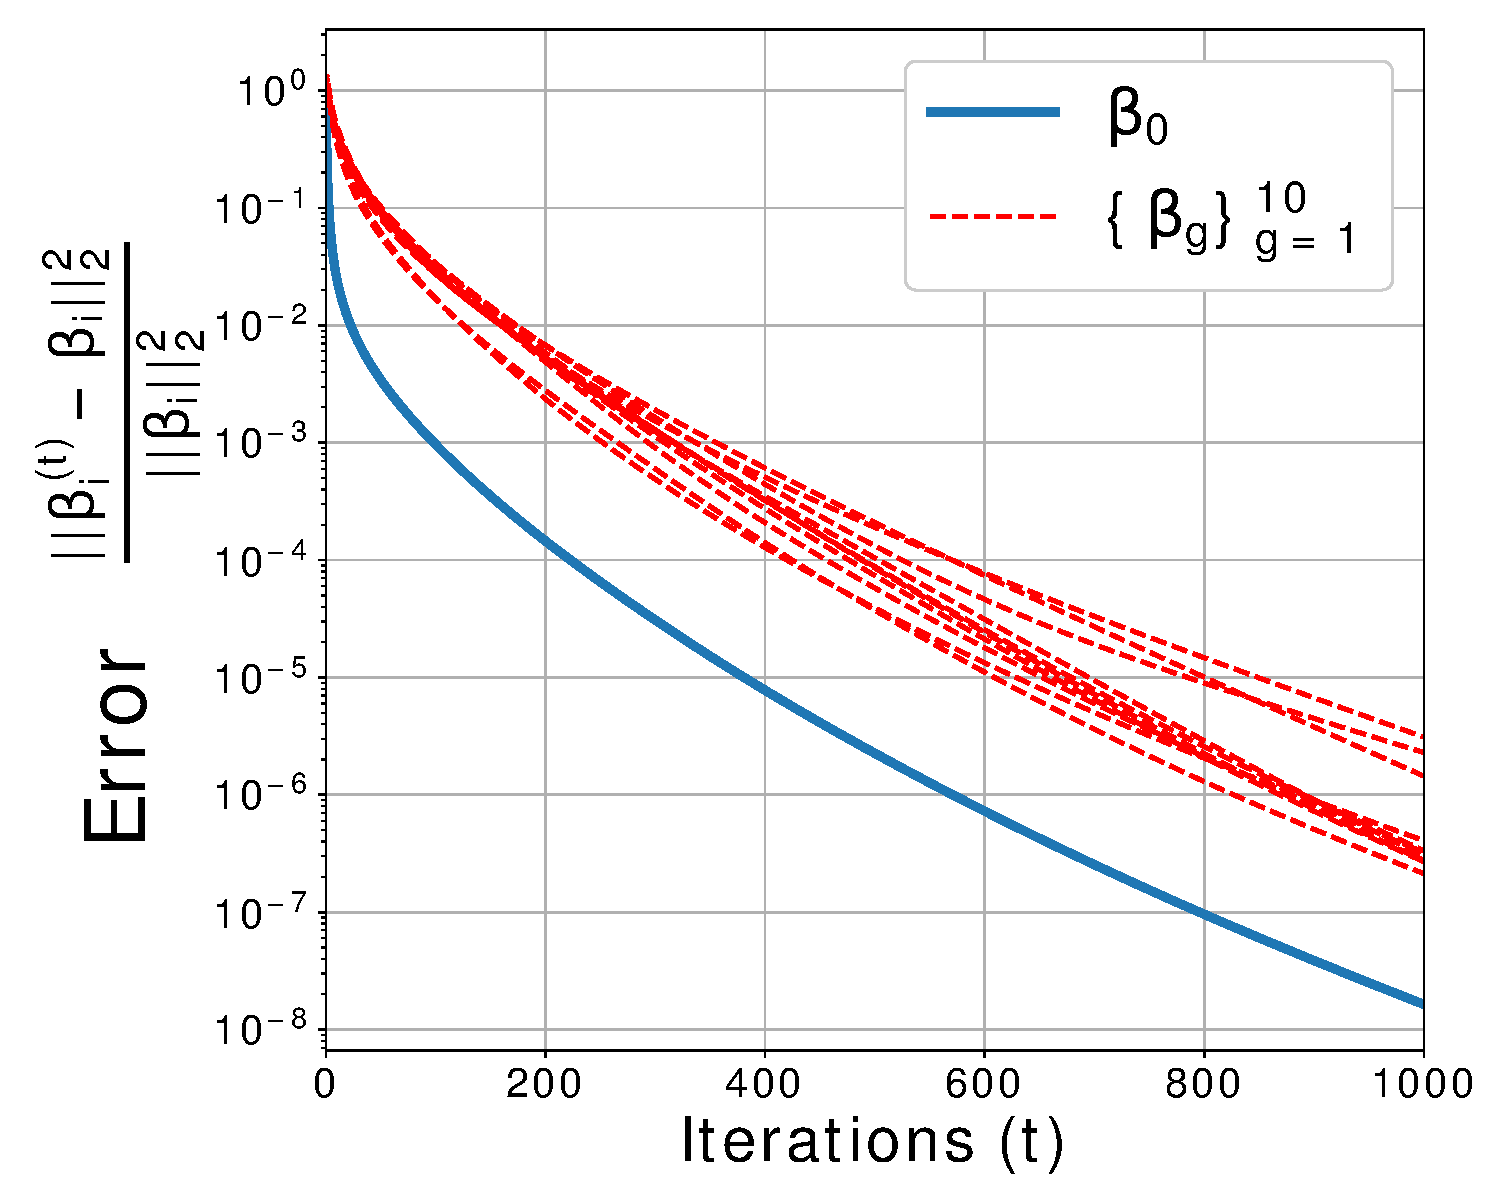
\includegraphics[width=\textwidth]{img/betag_converge_G10_p100.eps}
%			
%			\caption{}\label{fig syn1a}
%		\end{subfigure} ~
%		\begin{subfigure}[b]{0.5\textwidth}
%			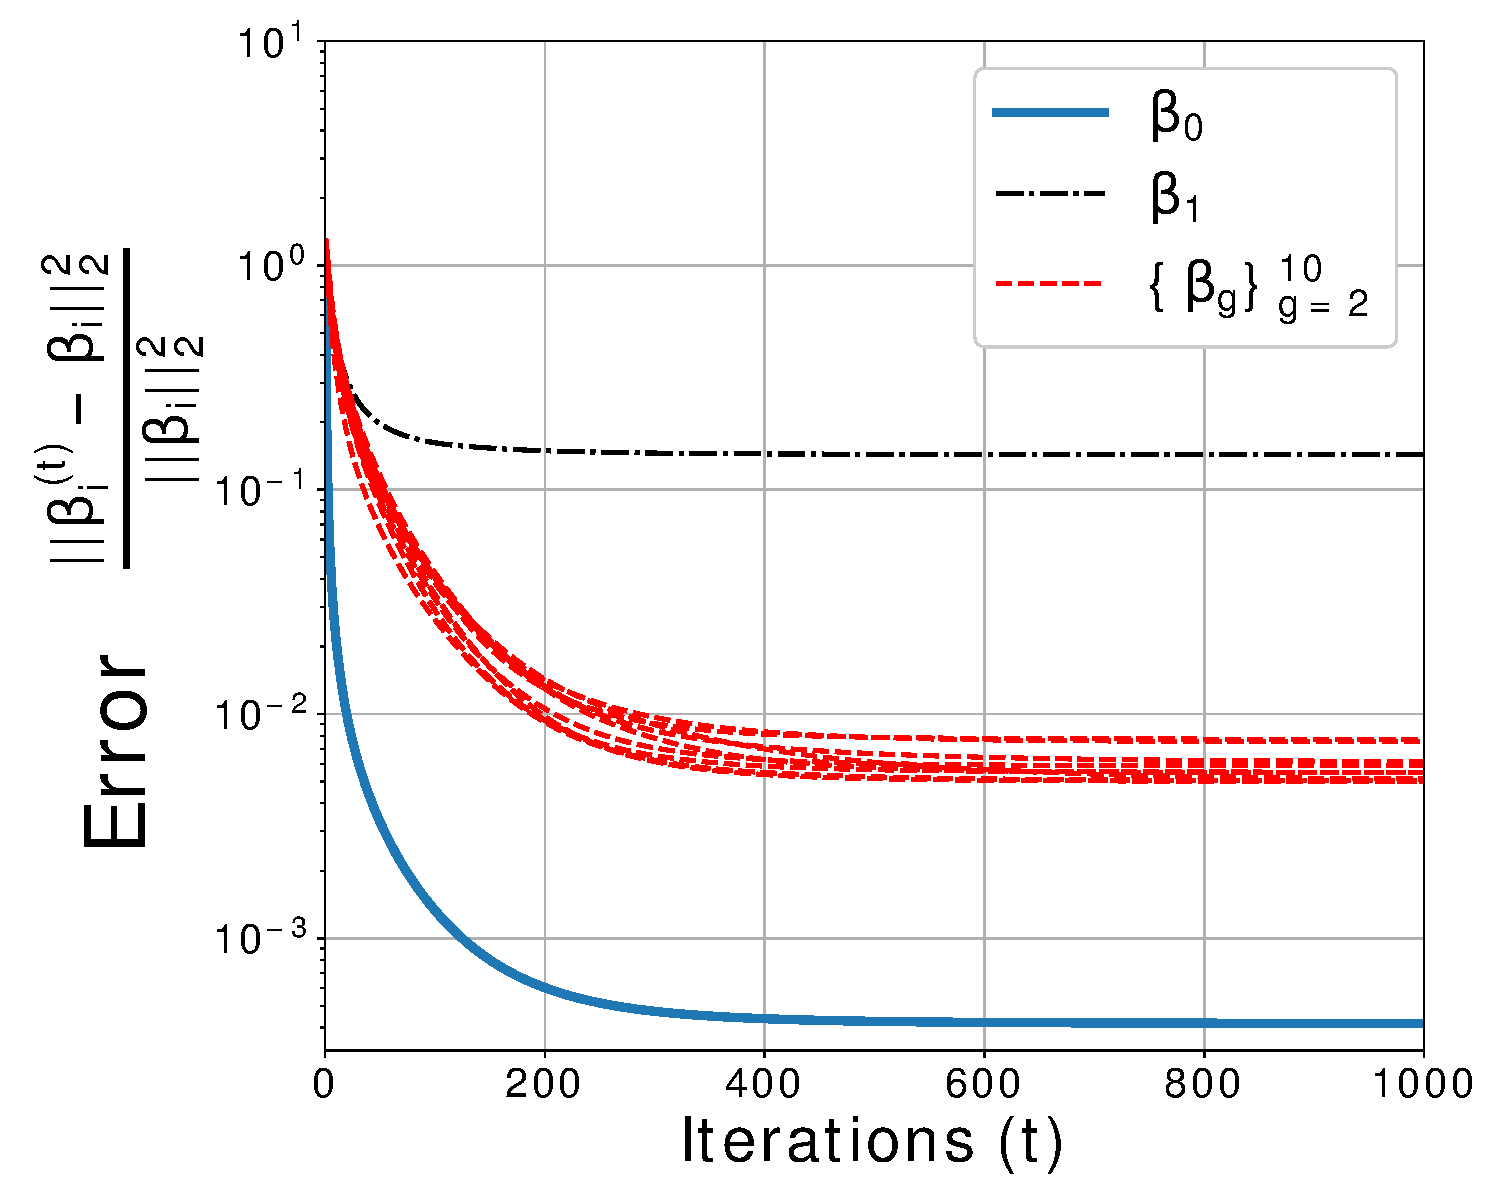
\includegraphics[width=\textwidth]{img/betag_converge_noise_G10_p100.eps}
%			
%			\caption{}\label{fig syn1b}
%		\end{subfigure}
%		\caption{a) Noiseless fast convergence. b) Noise on the first group does not impact other groups as much.}
%		\label{fig syn1}
%	\end{figure}
%	
%	\begin{figure}[t!]
%		\begin{subfigure}[b]{0.5\textwidth}
%			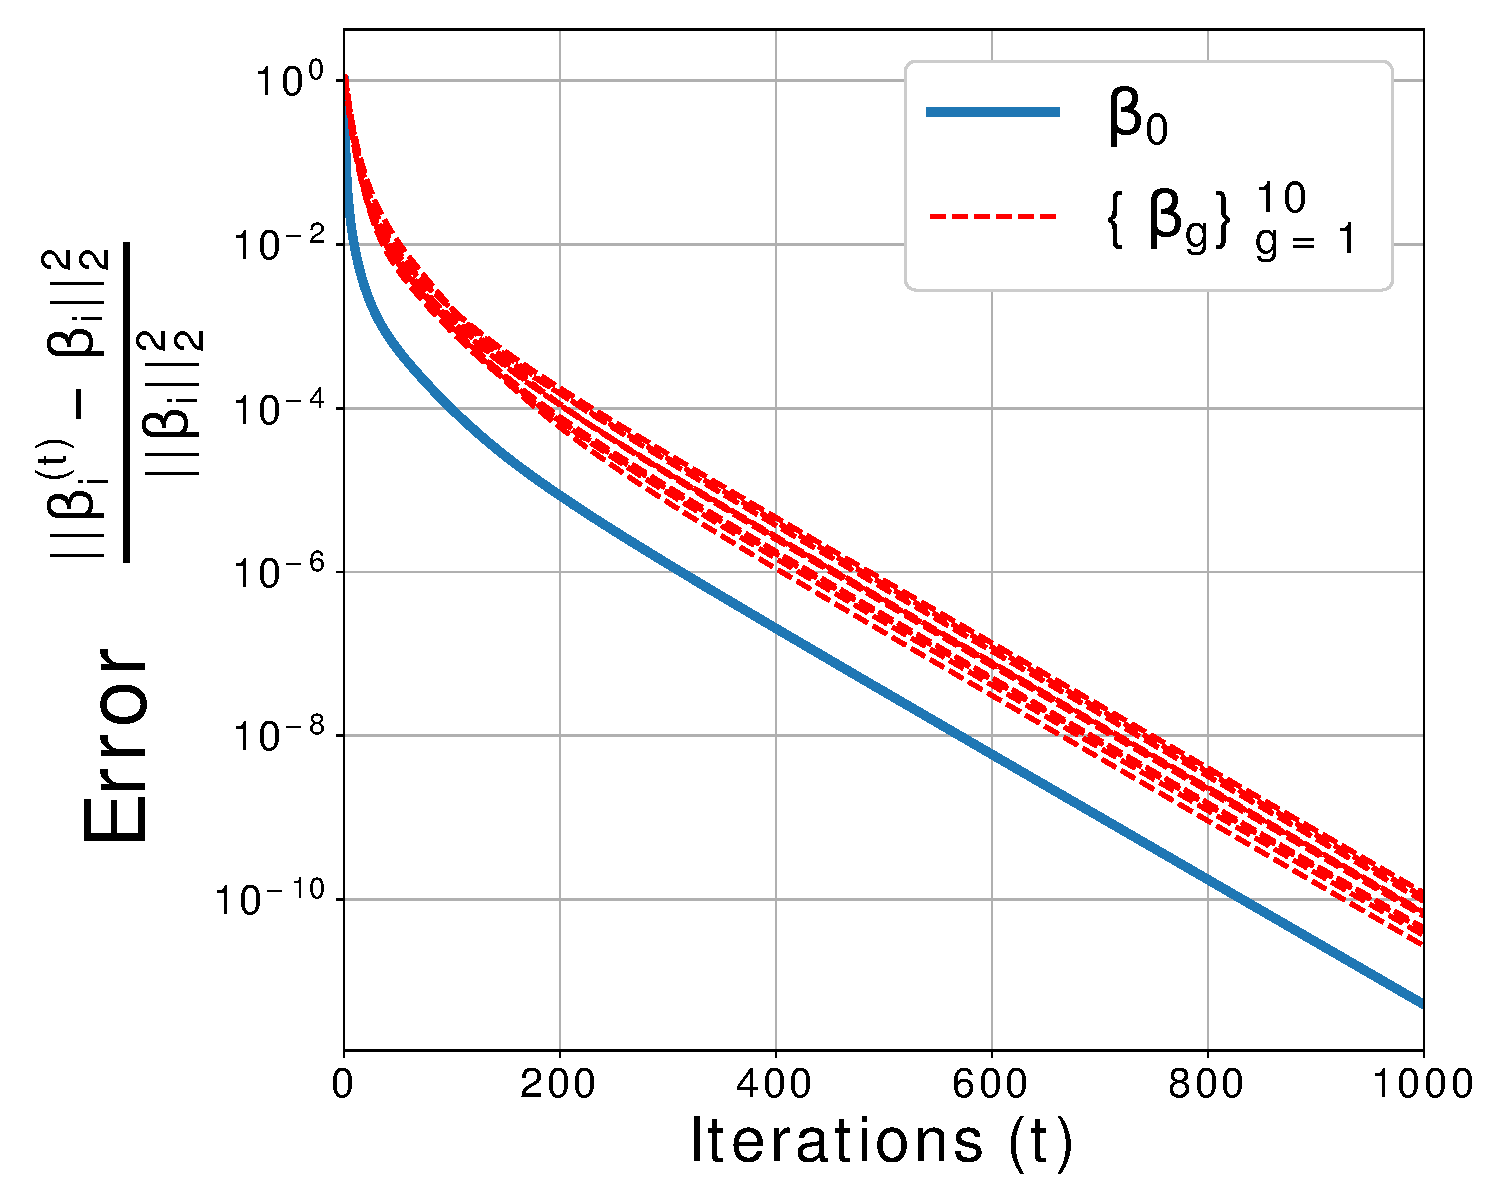
\includegraphics[width=\textwidth]{img/betag_converge_G10_p100_fast.eps}
%			
%			\caption{} \label{fig syn2a}
%		\end{subfigure} ~
%		\begin{subfigure}[b]{0.5\textwidth}
%			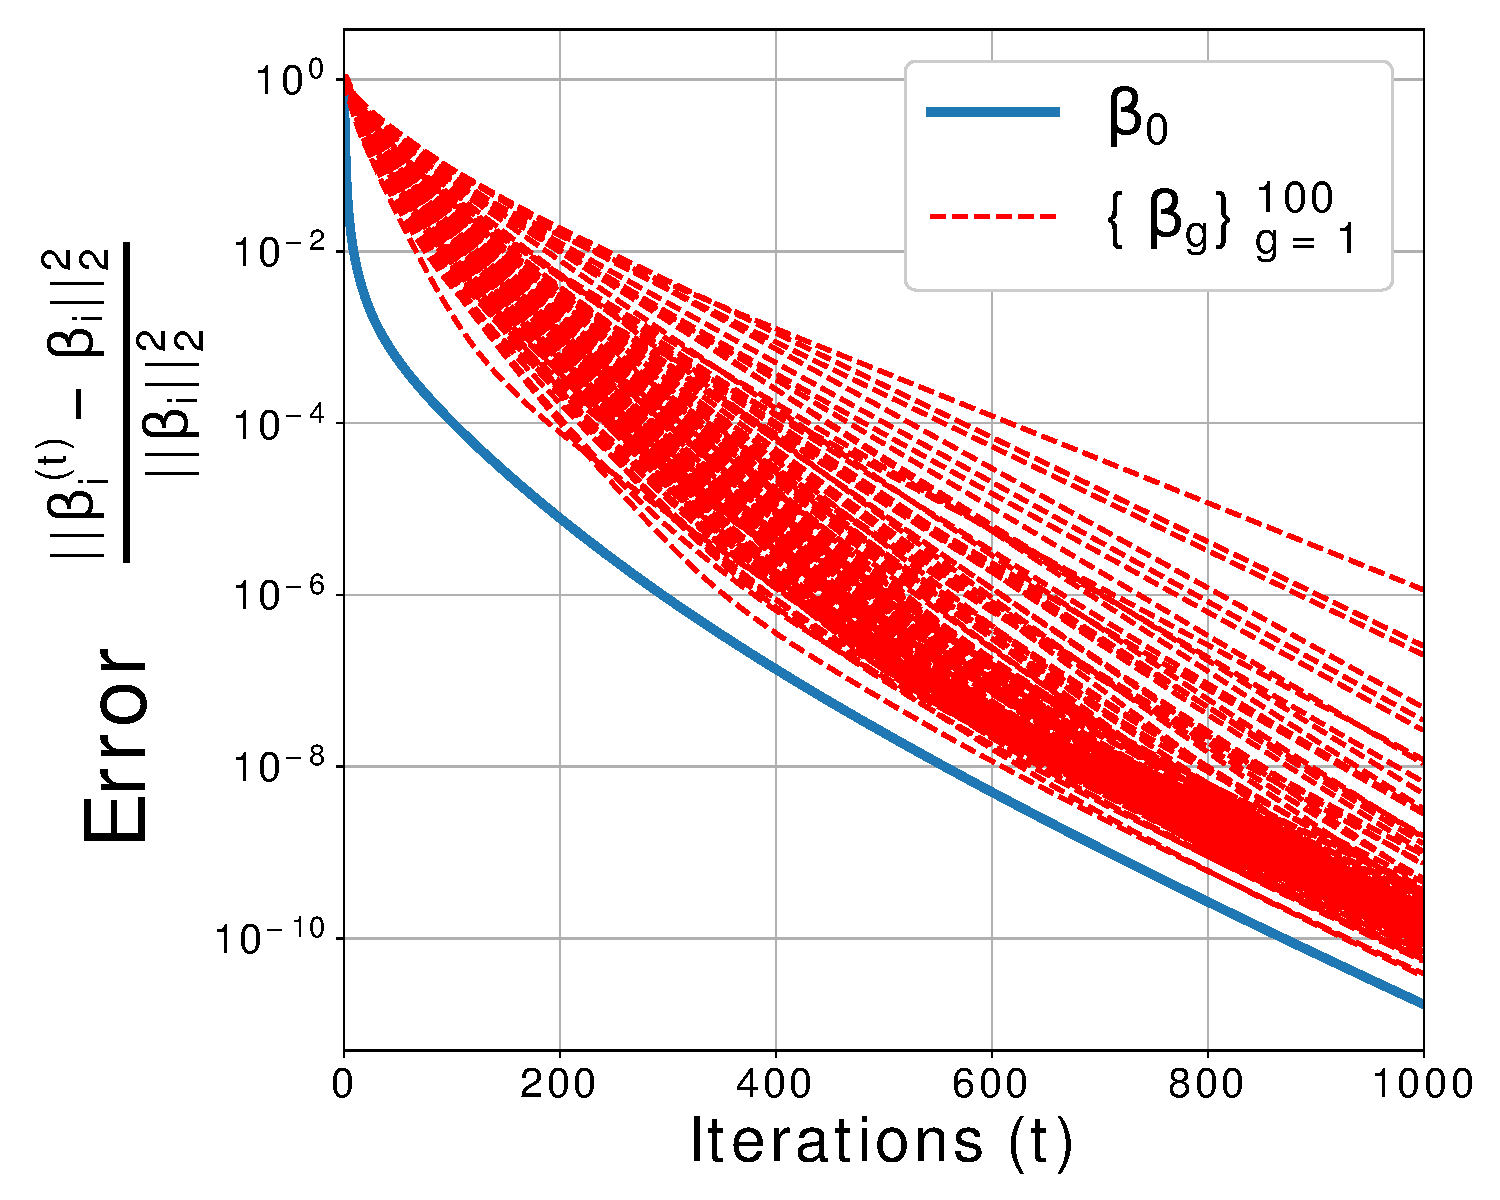
\includegraphics[width=\textwidth]{img/betag_converge_G100_p1000_shrink}
%			
%			\caption{}\label{fig syn2b}
%		\end{subfigure}
%		\caption{a) Increasing sample size improves rate of convergence. b) Our algorithm convergences fast even with a large number of groups $G=100$.}
%		\label{fig syn2}
%	\end{figure}

\vspace{5mm}

		\begin{figure}[t!]
			\centering
			\begin{subfigure}[b]{0.2175\textwidth}
				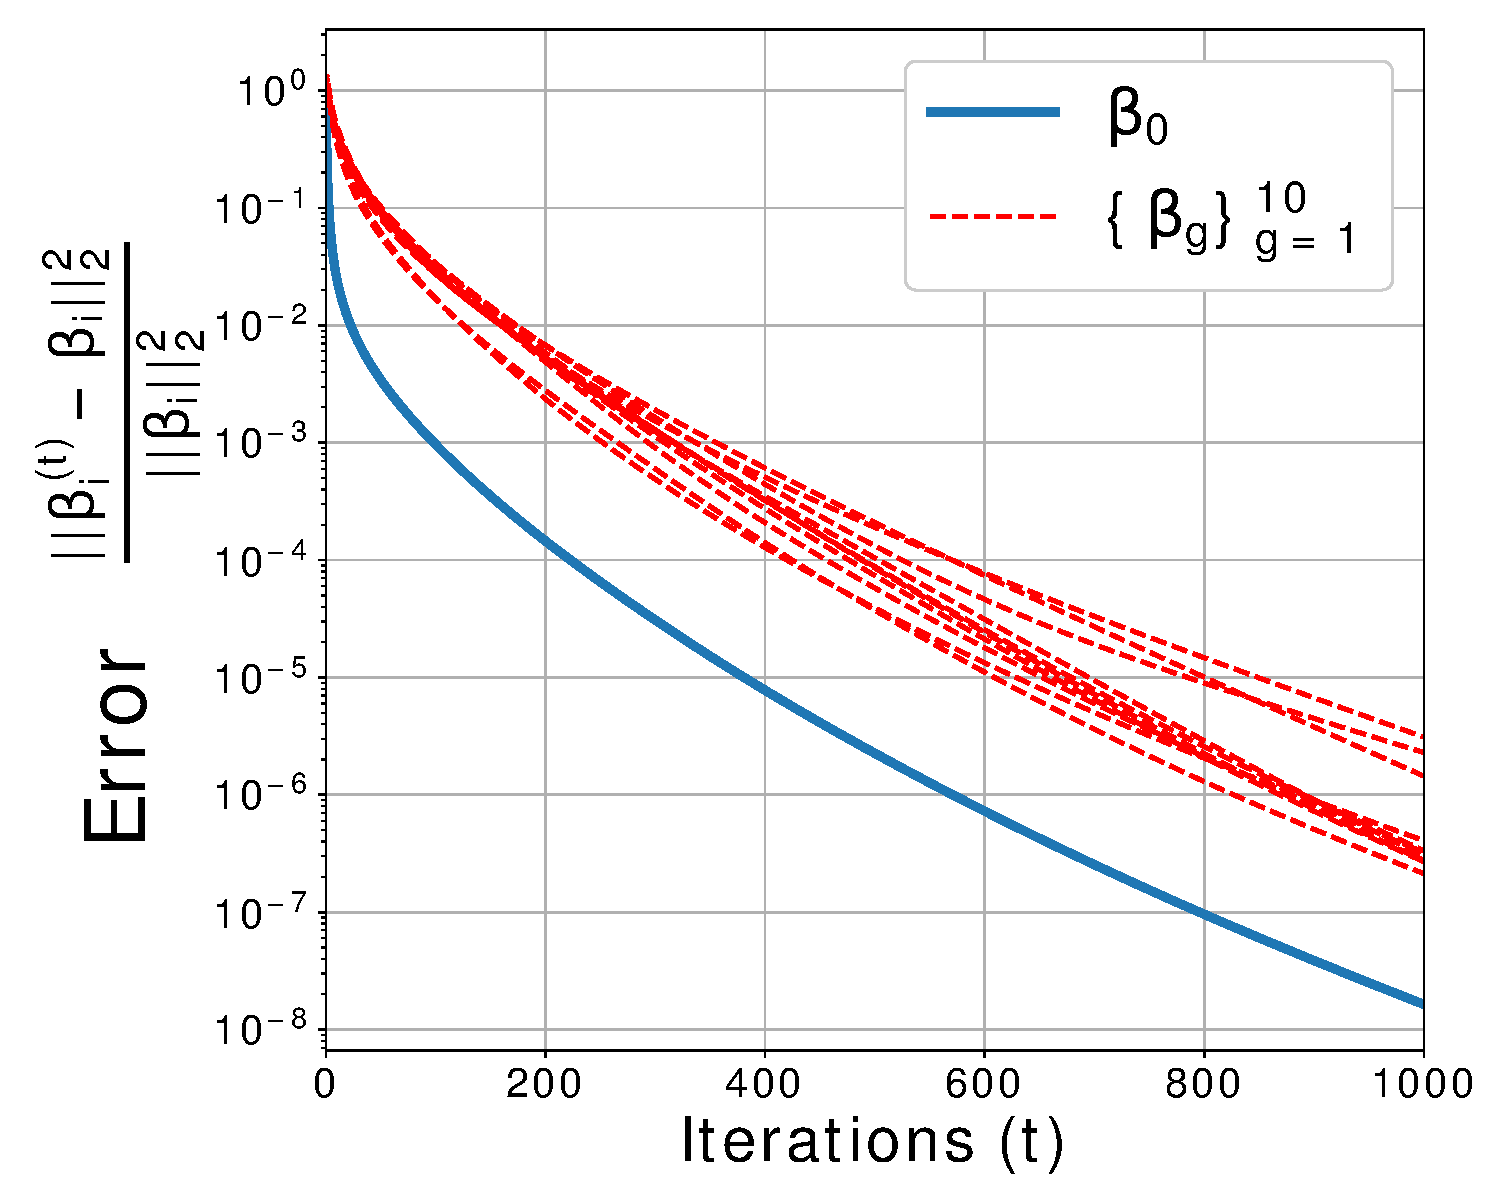
\includegraphics[width=\textwidth]{./img/betag_converge_G10_p100.pdf}				
				\caption{}\label{fig syn1a}
			\end{subfigure} ~
			\begin{subfigure}[b]{0.2175\textwidth}
				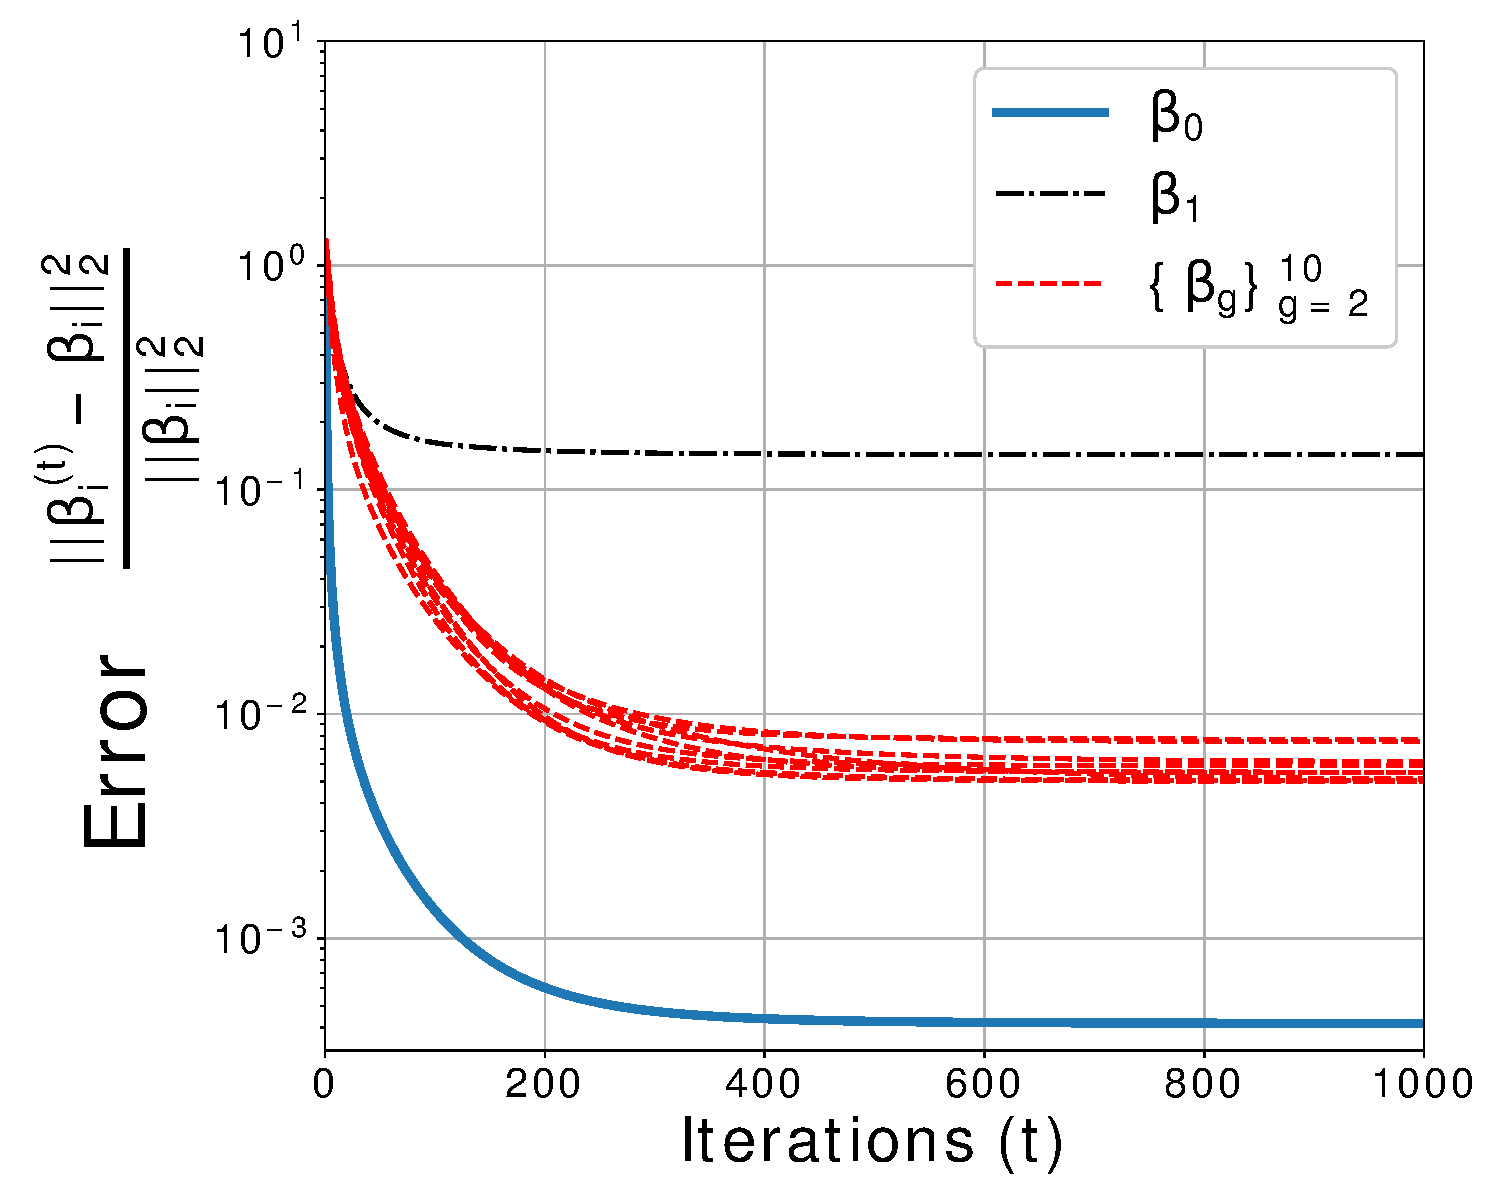
\includegraphics[width=\textwidth]{./img/betag_converge_noise_G10_p100.pdf}				
				\caption{}\label{fig syn1b}
			\end{subfigure}
%			\label{fig syn1}
			\begin{subfigure}[b]{0.2175\textwidth}
				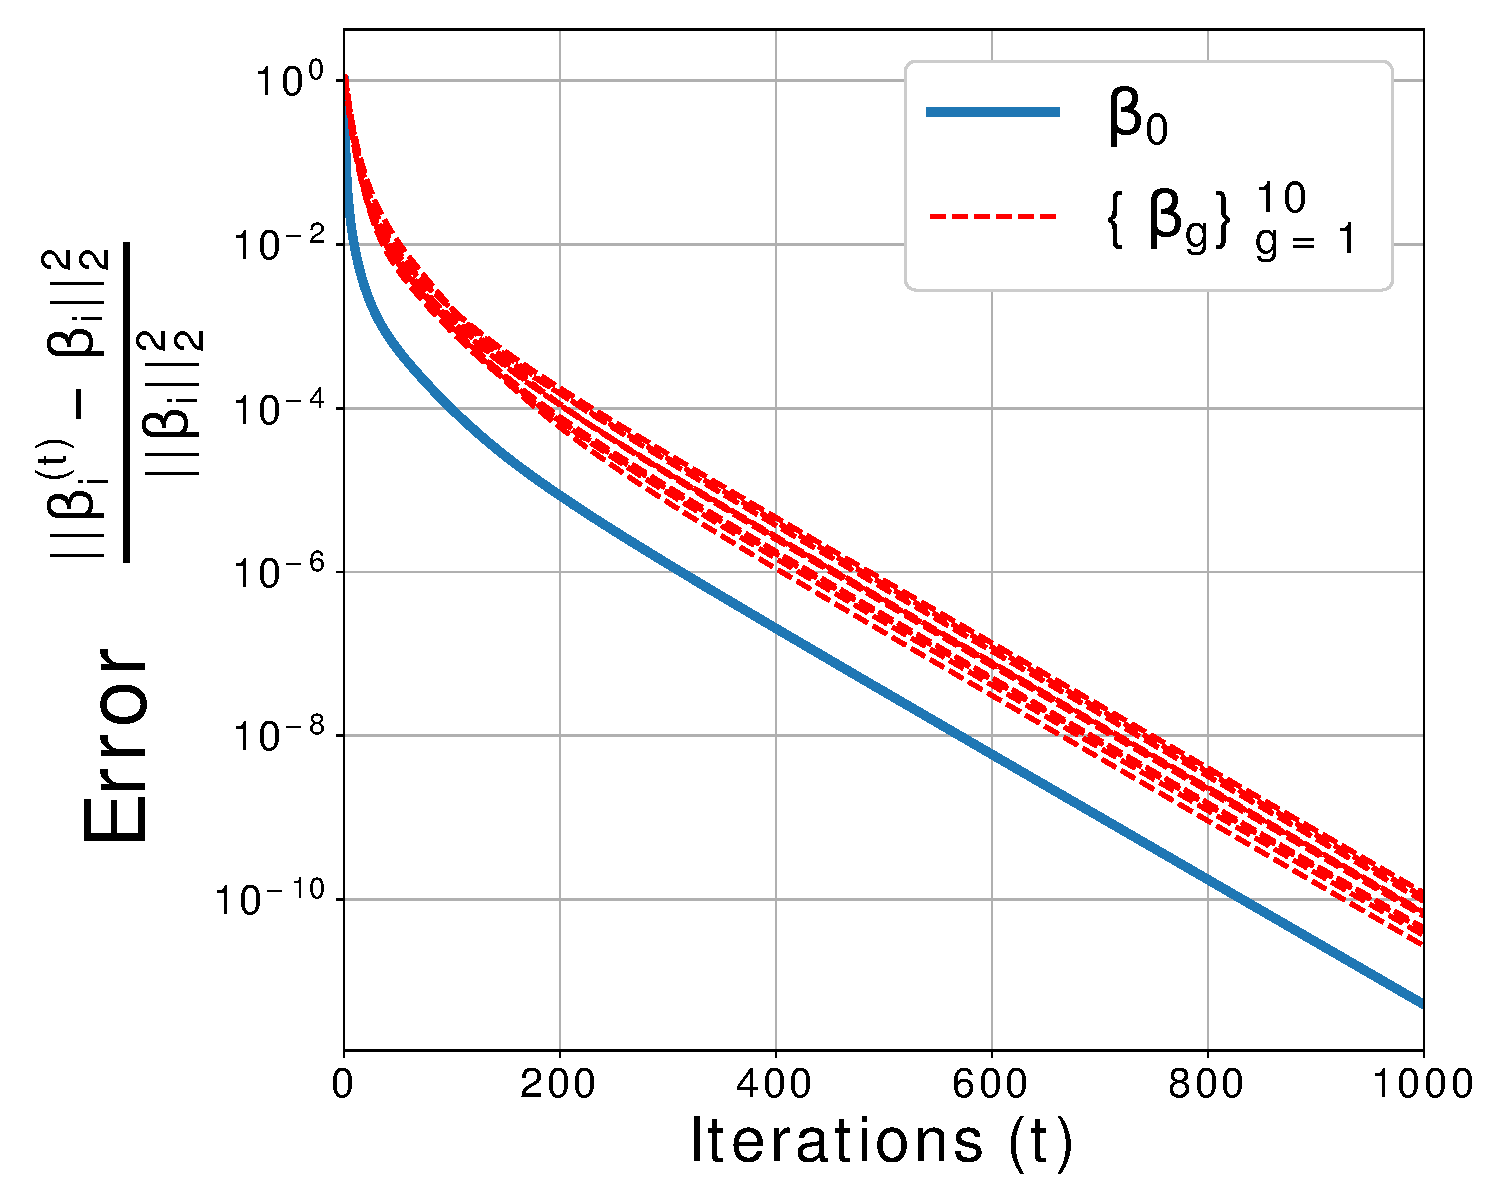
\includegraphics[width=\textwidth]{./img/betag_converge_G10_p100_fast.pdf}
				\caption{} \label{fig syn2a}
			\end{subfigure} ~
			\begin{subfigure}[b]{0.2175\textwidth}
				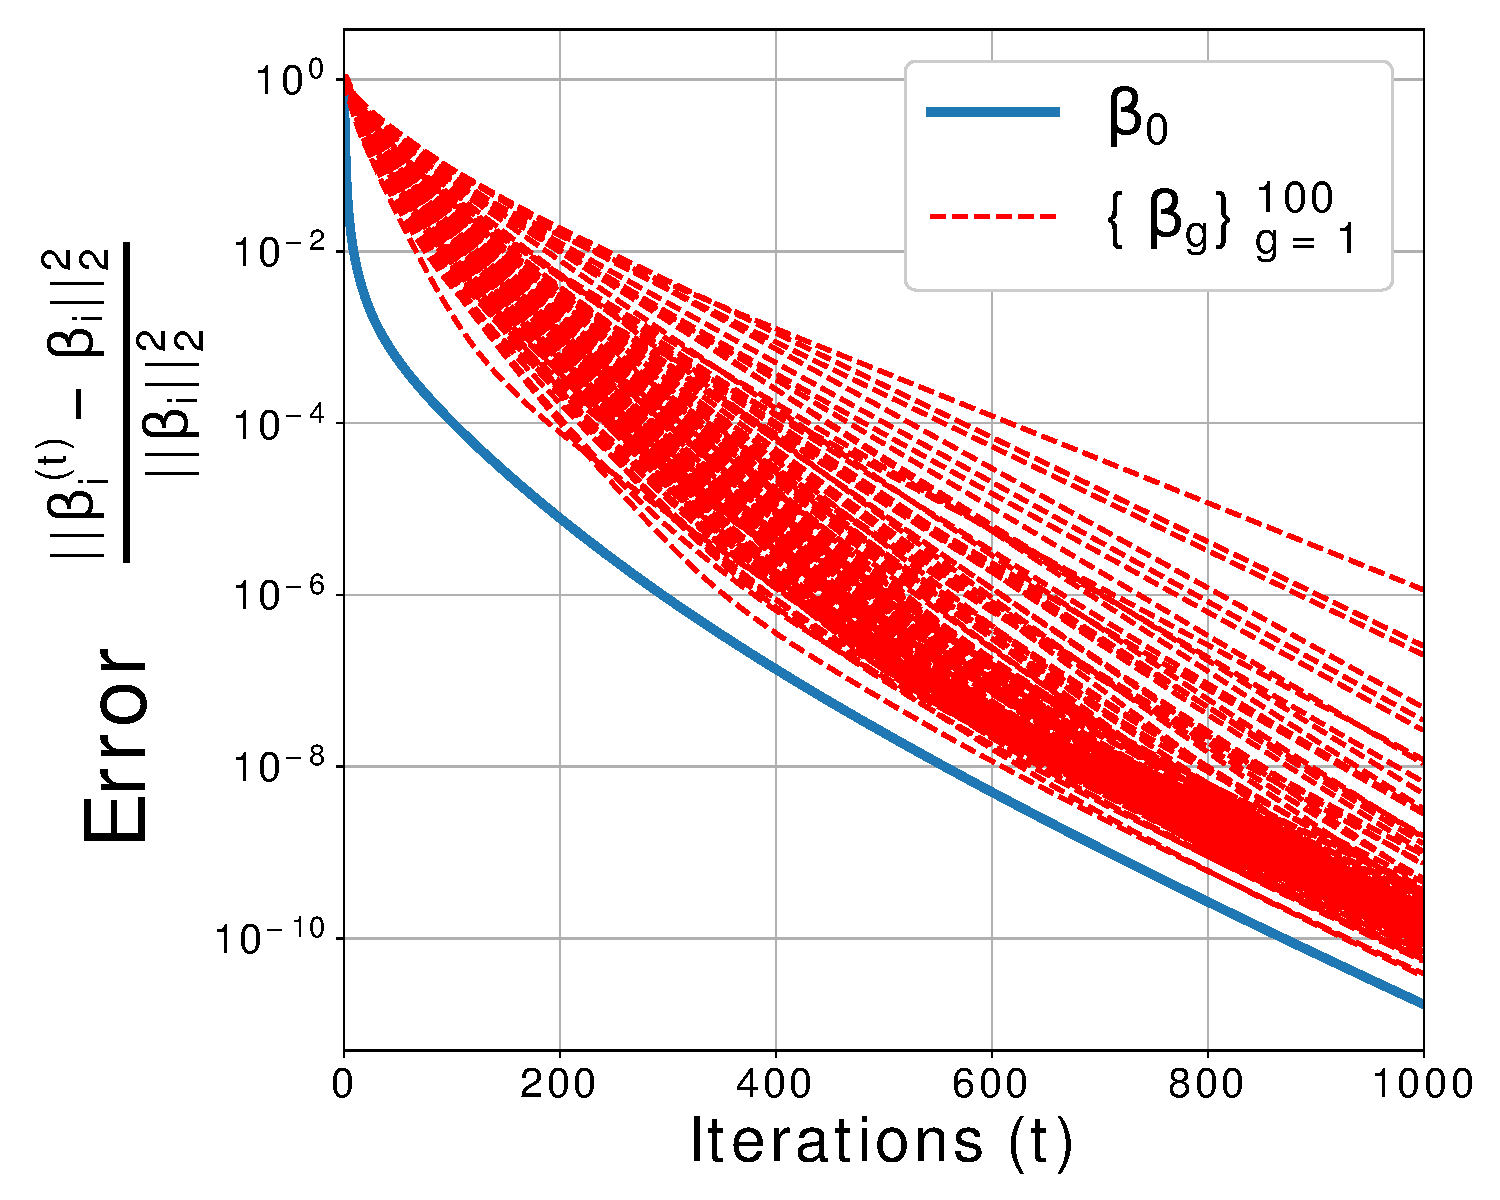
\includegraphics[width=\textwidth]{./img/betag_converge_G100_p1000_shrink.pdf}
				\caption{}\label{fig syn2b}
			\end{subfigure}
			\squeezeup
			\caption{a) Noiseless fast convergence. b) Noise on the first group does not impact other groups as much. c) Increasing sample size improves rate of convergence. d) Our algorithm convergences fast even with a large number of groups $G=100$.}
			\label{fig syn2}
		\end{figure}
	

%%%%%%%%%%%%% Amir's exp commented for now
%In this section we supplement our theoretical results with a simple synthetic experiment. 
%We focus on the case of two groups, i.e., $G = 2$. 
%The dimension $p = 1000$ and the structure is sparsity induced by $l_1$-norm. 
%The parameters $\bbeta _0^*$, $\bbeta _1^*$, and $\bbeta _2^*$ are 20, 10, and 5-sparse respectively. 
%The sparsity pattern is as follows:$\bbeta _0^* = (\underbrace{1, \dots, 1}_{1-20}, 0, \dots)$,$\bbeta _1^* = (\dots, 0, \underbrace{2, \dots, 2}_{51-60}, 0, \dots)$, and $\bbeta _2^* = (\dots, 0, \underbrace{-2, \dots, -2}_{96-100}, 0, \dots)$. 
%
%For the distribution of input and noise we have $\x_{gi} \sim N(0, \sigma_x^2 \I)$ and $\omega_{gi} \sim N(0, \sigma_w^2)$ with $\sigma_x^2 = .3$ and  $\sigma_w^2 = .1$.
%We use the SPGD method (Algorithm \ref{alg2}) to solve the optimization problem \eqref{eq:compact}. 
%The projection to the $l_1$ ball can be efficiently performed by the method proposed in \cite{dssc08}. 
%
%While changing $n$ in the experiments, we keep the ratio $\frac{n_1}{n_2} = \frac{2}{3}$ fixed. 
%Figures \ref{fig:individual1} and \ref{fig:individual2} show the per-group error for different sample size which follows $1/\sqrt{n_g}$ decay.
%Finally, Figure \ref{fig:common} shows the decay of the error as sample size increases for the common component recovery and the error for summation of the form \eqref{eq:errorsum}.
%As expected errors decay as $1/\sqrt{n}$.
%
%\begin{figure}
%	\centering
%	\subcaptionbox{
%		Individual parameter one.
%		\label{fig:individual1}
%	}{\includegraphics[width=0.3 \textwidth]{./img/synthbeta1}}~
%	\subcaptionbox{
%		Individual parameter two.
%		\label{fig:individual2}
%	}{\includegraphics[width=0.3 \textwidth,]{./img/synthbeta2}}
%	\subcaptionbox{
%		Common parameter.
%	\label{fig:common}
%	}{\includegraphics[width=0.3 \textwidth,]{./img/synthbeta0}}
%	\caption{Estimation error with different sample size. Each point on the diagram is an average over 30 experiments.} %\ref{fig:common} compares the error with the LHS of \eqref{eq:errorsum}
%	\label{fig:gasprices}
%\end{figure}

\vspace{-10mm}
\section{Anti-Cancer Drug Sensitivity Prediction}
\label{realexp}
In this section, we investigate the application of \dc{} in analyzing the response of cancer tumor cell lines to different doses of various drugs. 
Each cancer type (lung, blood, etc.) is a group $g$ in our DE model and the respond of patient $i$ with cancer $g$ to the drug is our output $y_{gi}$. 
The set of features for each patient $\x_{gi}$ consists of gene expressions, copy number variation, and mutations and $y_{gi}$ is the ``activity area'' above the dose-response curve, Figure \ref{fig:dr}.
Given $\x_{gi}$ and a drug, we have two goals: accurately predict a patient's response to the drug and identifying genetic predictors of drug sensitivity. 
%We present more details about and results of the drug sensitivity experiment in Appendix \ref{?}.
%In other words, we are interested in both predicting of $y_{gi}$ and identifying feature $j$ with highest absolute $\bbeta_{g}(j)$ value for each cancer $g$.
%We hope that the data enriched model captures the important shared feature between cancers, as long as the cancer-specific genetic factors that determine the response to therapy.
%In the following, we first explain the dataset and then compare the prediction performance of DS with elastic net on 24 drugs. 
%Then, we perform a more detailed study of the features selected by DS to validate if DS extracts meaningful feature for each cancer. 
%\subsection{Data Set}
%A dose-response dataset of an anticancer drug $d$ and a cell line $gi$ (sampled from a patient $i$ with cancer $g$) consists of pairs ${(c, p)}$ which means proportion $p$ of cells of the cell line $gi$ are alive (relative viability) when treated with drug $d$ with concentration $c$. 
%%There are many methods that fit different function to dose-response data, 
%When a drug \emph{works}, after fitting a function to raw data, we will have a reverse sigmoid-like graph, e.g., Figure \ref{fig:dr}. 
%An effective drug kills more cells with lower concentrations therefore its  ``activity area'' \cite{zoha05}, i.e., area above the curve in Figure \ref{fig:dr}, is larger.
%%There are many ways to measure the drug efficacy from the dose-response curve. 
%We use the activity area of the drug for cell line $gi$ as our output of interest $y_{gi}$. 
%
%\begin{figure}
%	\centering
%	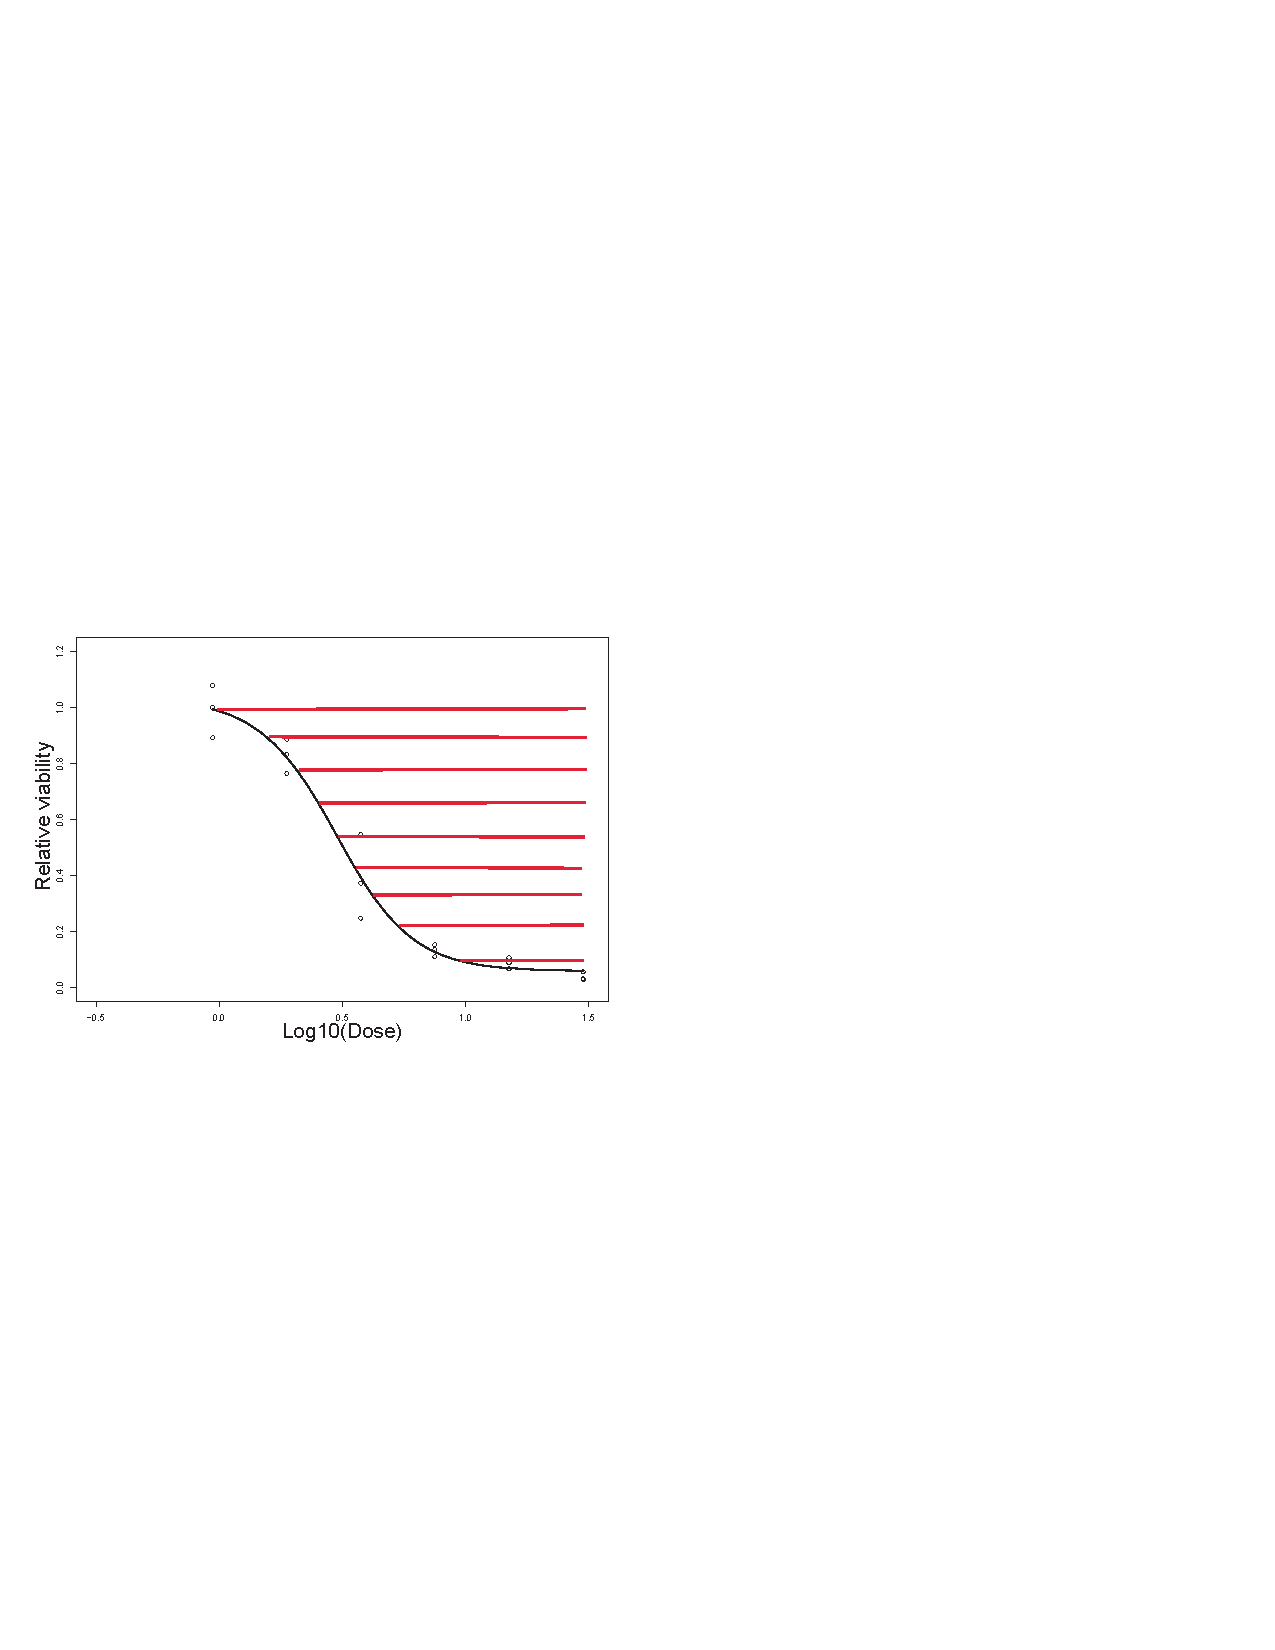
\includegraphics[width=0.3 \textwidth,]{./img/dr4}
%	\caption{}
%	\label{fig:dr}
%\end{figure}

%In this experiment 
We use Cancer Cell Line Encyclopedia (CCLE) \cite{barretina2012cancer} which is a compilation $\sim$500 human cancer cell lines where their responses to 24 anticancer drugs have been measured.%\footnote{Here the technical meaning of response $y_{gi}$ is the ``activity area'' above the dose-response curve\cite{barretina2012cancer}.}.
%The goal of the study was to identify genetic predictor of drug sensitivity for different cancers. 
%The method used for analysis of CCLE in the original paper was Elastic Net \cite{zoha05} which we use as the comparison baseline. 
%\footnote{Cancer type is the first tissue where the cancer was observed.} 
We perform two \emph{experiments} where the number of cancers in each data set are $G =2$ or $3$ and we name them TWO and THREE experiments, respectively. 
We consider lung and blood\footnote{By blood cancer, we mean any cancer originate from haematopoietic and lymphoid tissues.} for TWO while for THREE we predict the drug sensitivity of skin, breast and ovary cancer cell lines. 
Beyond these five cancer types, others have less than 50 samples, so we remove them from consideration.
Each experiment consists of 24 \emph{problems} each corresponds to a drug. % drug sensitivity prediction of 
Not all of the $~$500 cell lines have been treated with all of the drugs. 
Therefore each problem has a different number of samples $n$ where $n \in [90, 160]$ for TWO and $n \in [70, 100]$ for THREE experiments.
We perform a standard preprocessing \cite{barretina2012cancer} where we remove features with less than $.2$ absolute correlation with the response of interest.% which reduces the dimension from $>30,000$ to $p \in [?, ?]$.% range. 
Note that the features that get removed vary by problem, therefore the dimension $p$ is reduced from from $>30,000$ to $p \in [1000, 15000]$. 

%\subsection{Results}
{\bf Prediction:} In each TWO and THREE experiments, we predict the drug sensitivity for 24 different drugs.  %= \{f_g(\bbeta) < b_g\}$
Since the values of $d_g$  in constraint sets $\Omega_{f_g}(d_g)$  are unknown, we tune them by 5-fold cross-validation and report the mean squared error (MSE) of \dc{} and a baseline method. 
Our \emph{baseline} method BL is the LASSO \cite{tibs96} equivalent of DE where we set $\forall g \in [G]_\setminus d_g = 0$ and only estimate the common parameter $\bbeta_0$. 
Figure \ref{fig:two} and \ref{fig:three} illustrate the performance of \dc{} and BL for TWO and THREE experiments respectively. 
Note that \dc{} outperforms BL in 21 and 18 out of 24 problems in TWO and THREE experiments, respectively.

To ensure that the prediction improvement of \dc{} over the baseline is significant, we supplement our analysis with the bootstrapped error of both methods for the TWO experiment.
For each problem in the TWO experiment, we generate 100 bootstrapped data sets by sampling with replacement as $\{(\X^{(i)}_{\text{TWO}}, \y^{(i)}_{\text{TWO}})\}_{i=1}^{100}$.  
Then, we fix $d_g$s hyper-parameters to values determined by cross-validation in the last stage and run both methods and compute pairs of MSEs as $\{(\text{MSE}^{(i)}_{\text{\dc}}, \text{MSE}^{(i)}_{\text{BL}})\}_{i=1}^{100}$. We perform paired t-test to determine if mean difference between MSEs is significant. In 21 out of 24 problems \dc's MSE is lesser than BL's with significance level of $\alpha = 0.05$. A representative set of results is demonstrated in Figure \ref{fig:allbars}. 

	\begin{figure}
	\centering
	\begin{subfigure}[b]{0.22\textwidth}
		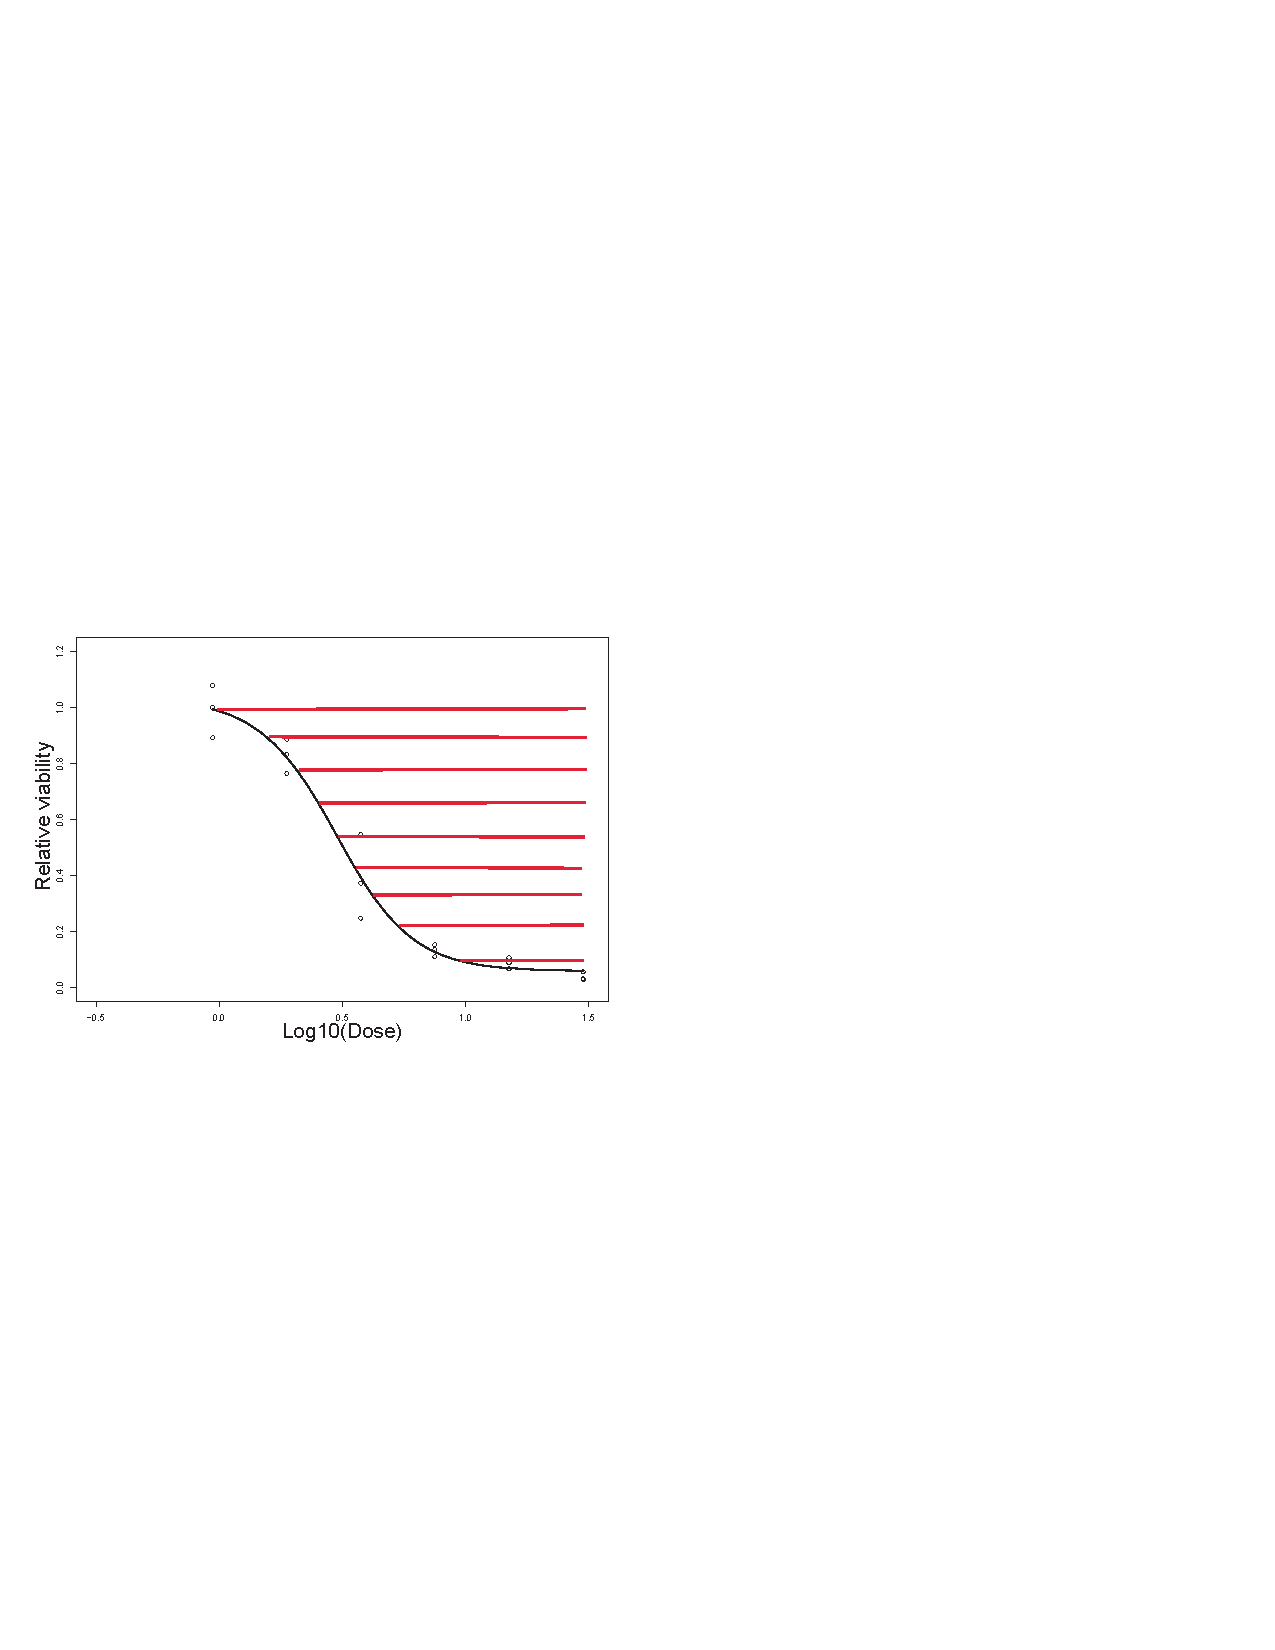
\includegraphics[width=\textwidth]{./img/dr4.pdf}
		\caption{}\label{fig:dr}
	\end{subfigure} ~
	\begin{subfigure}[b]{0.22\textwidth}
	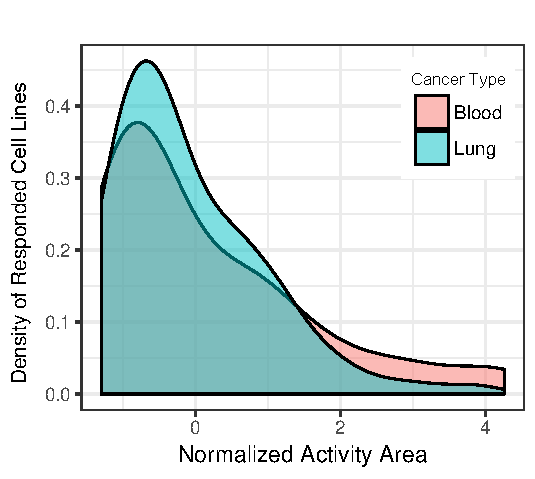
\includegraphics[height=2.65cm]{./img/Saracatinib.pdf}
	\caption{}\label{fig:Saracatinib}
	\end{subfigure}
	\squeezeup
	\caption{a) A sample fitted dose-response curve where Activity Area $y_{gi}$ is shaded. b) Distribution of responses to Saracatinib for which some lung and blood cancer cell lines have responded.}
	\label{fig syn2}
	\end{figure}


	\begin{figure}
	\centering
	\begin{subfigure}[b]{0.22\textwidth}
		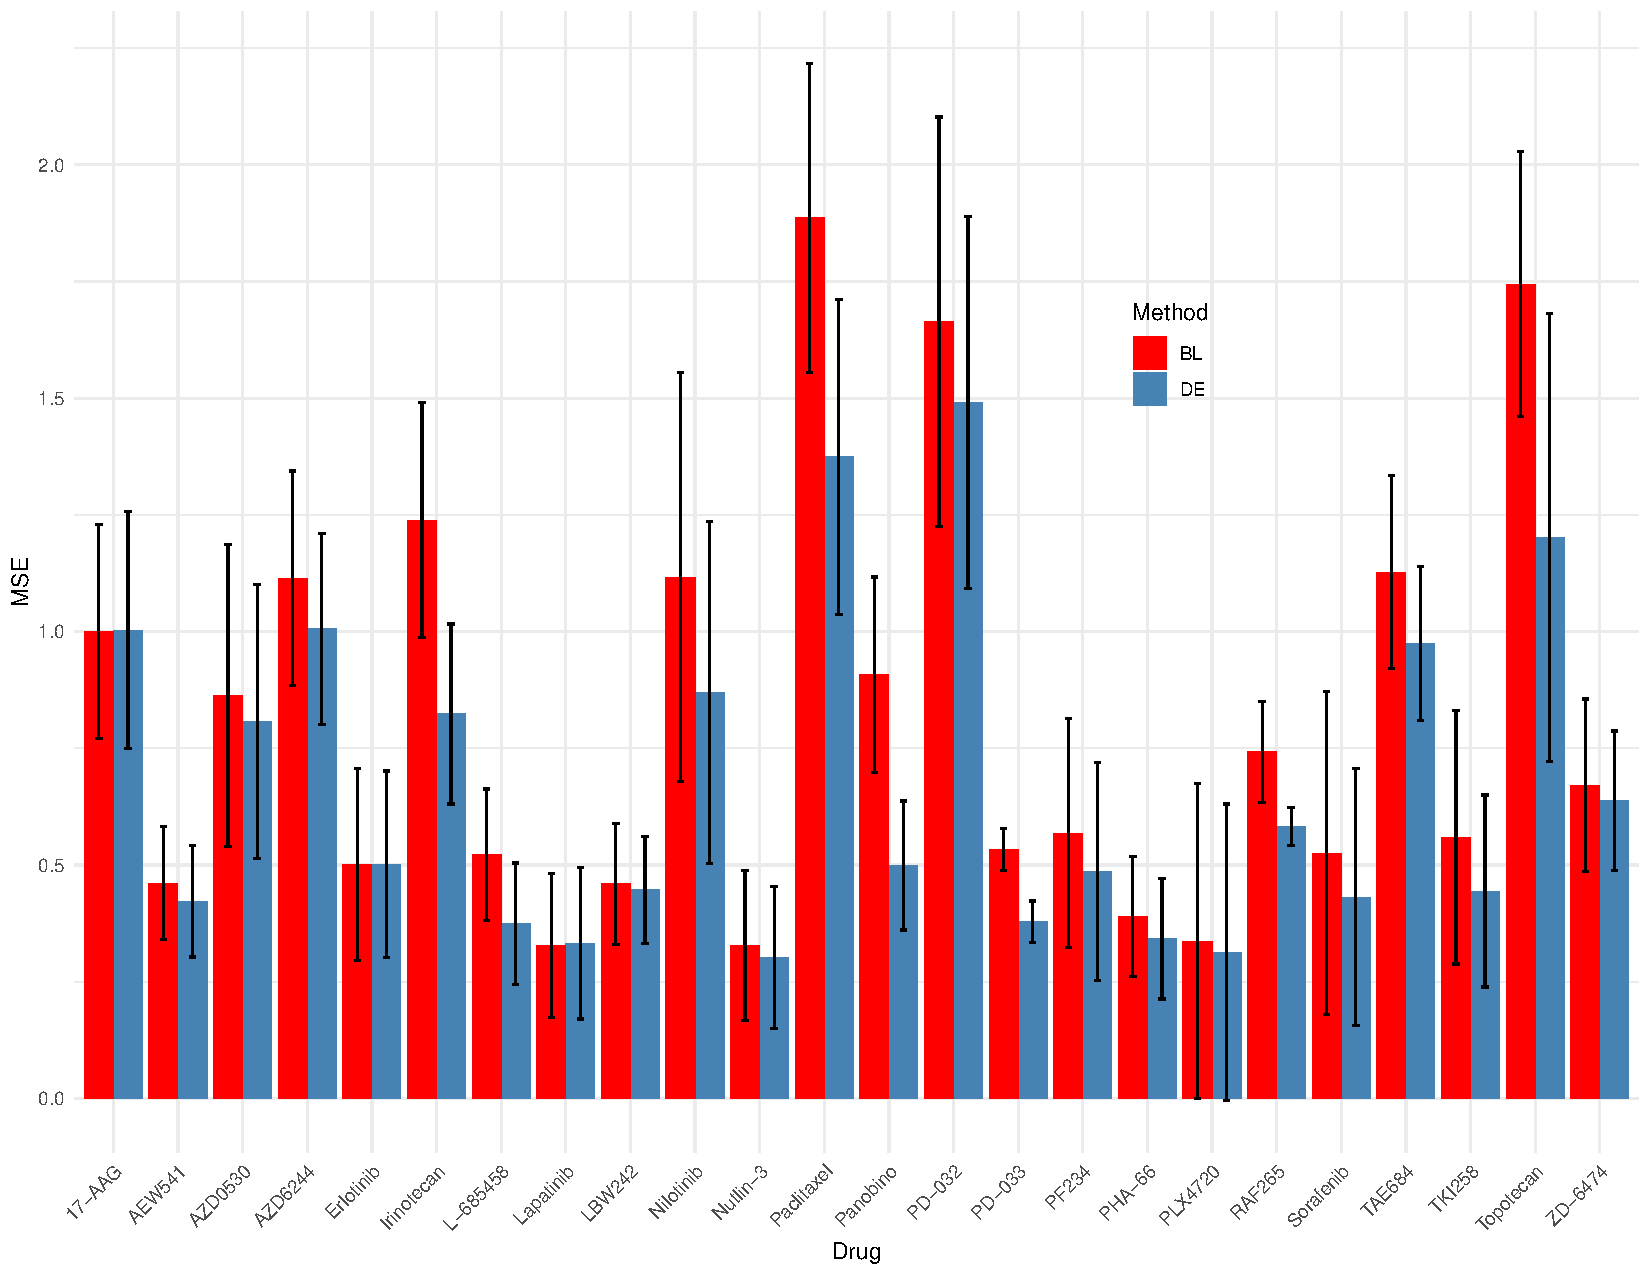
\includegraphics[width=\textwidth]{./img/lung-blood-barplot.pdf}
		\caption{Lung and Blood}\label{fig:two}
	\end{subfigure} ~
	\begin{subfigure}[b]{0.22\textwidth}
		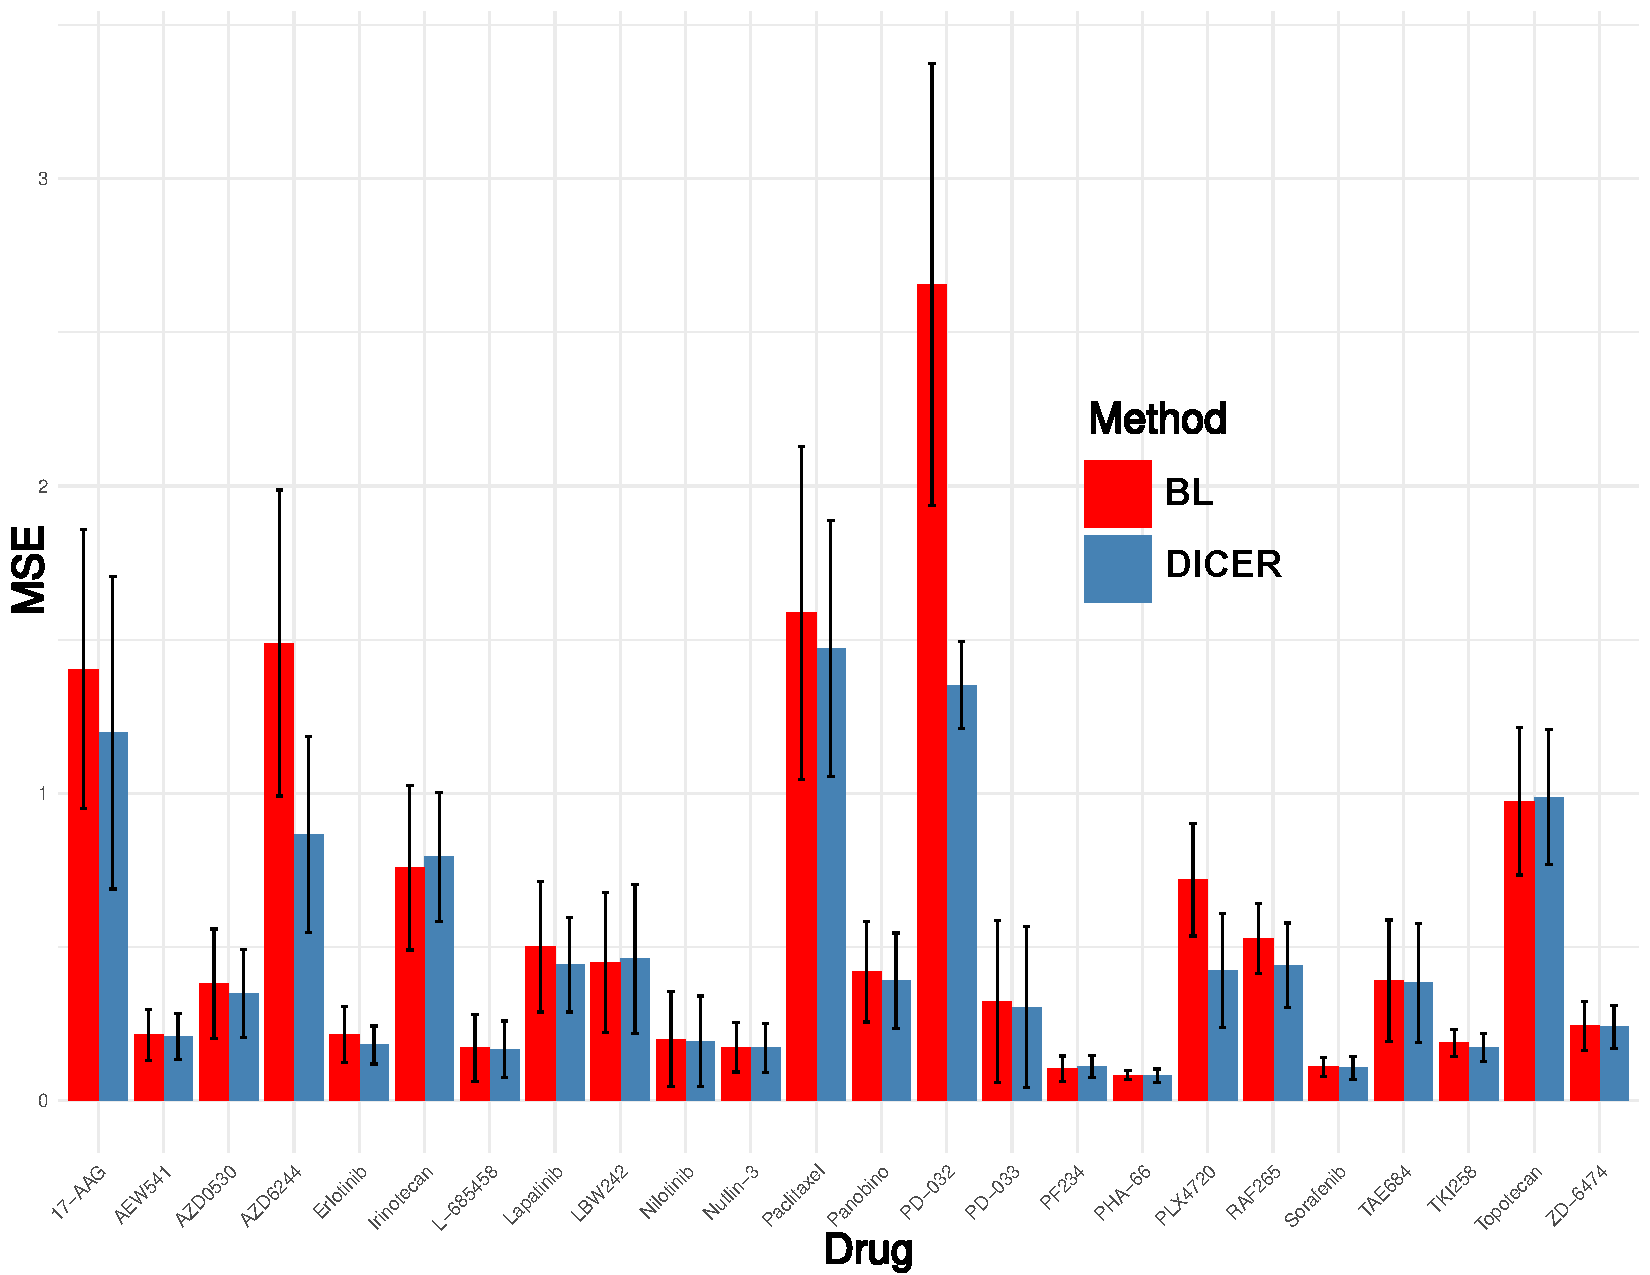
\includegraphics[width=\textwidth]{./img/skin-ovary-breast.pdf}
		\caption{Skin, Ovary, and Breast}\label{fig:three}
	\end{subfigure}
	\squeezeup
	\caption{Distribution of MSE Comparison of Mean Square Error of \dc{} and BL in predicting the response to 24 drugs in TWO and THREE experiments. Each bar is the mean of MSE for 5-fold cross-validation.}
	\label{fig syn2}
\end{figure}

	\begin{figure}
	\centering
	\begin{subfigure}[b]{0.22\textwidth}
		\centering
		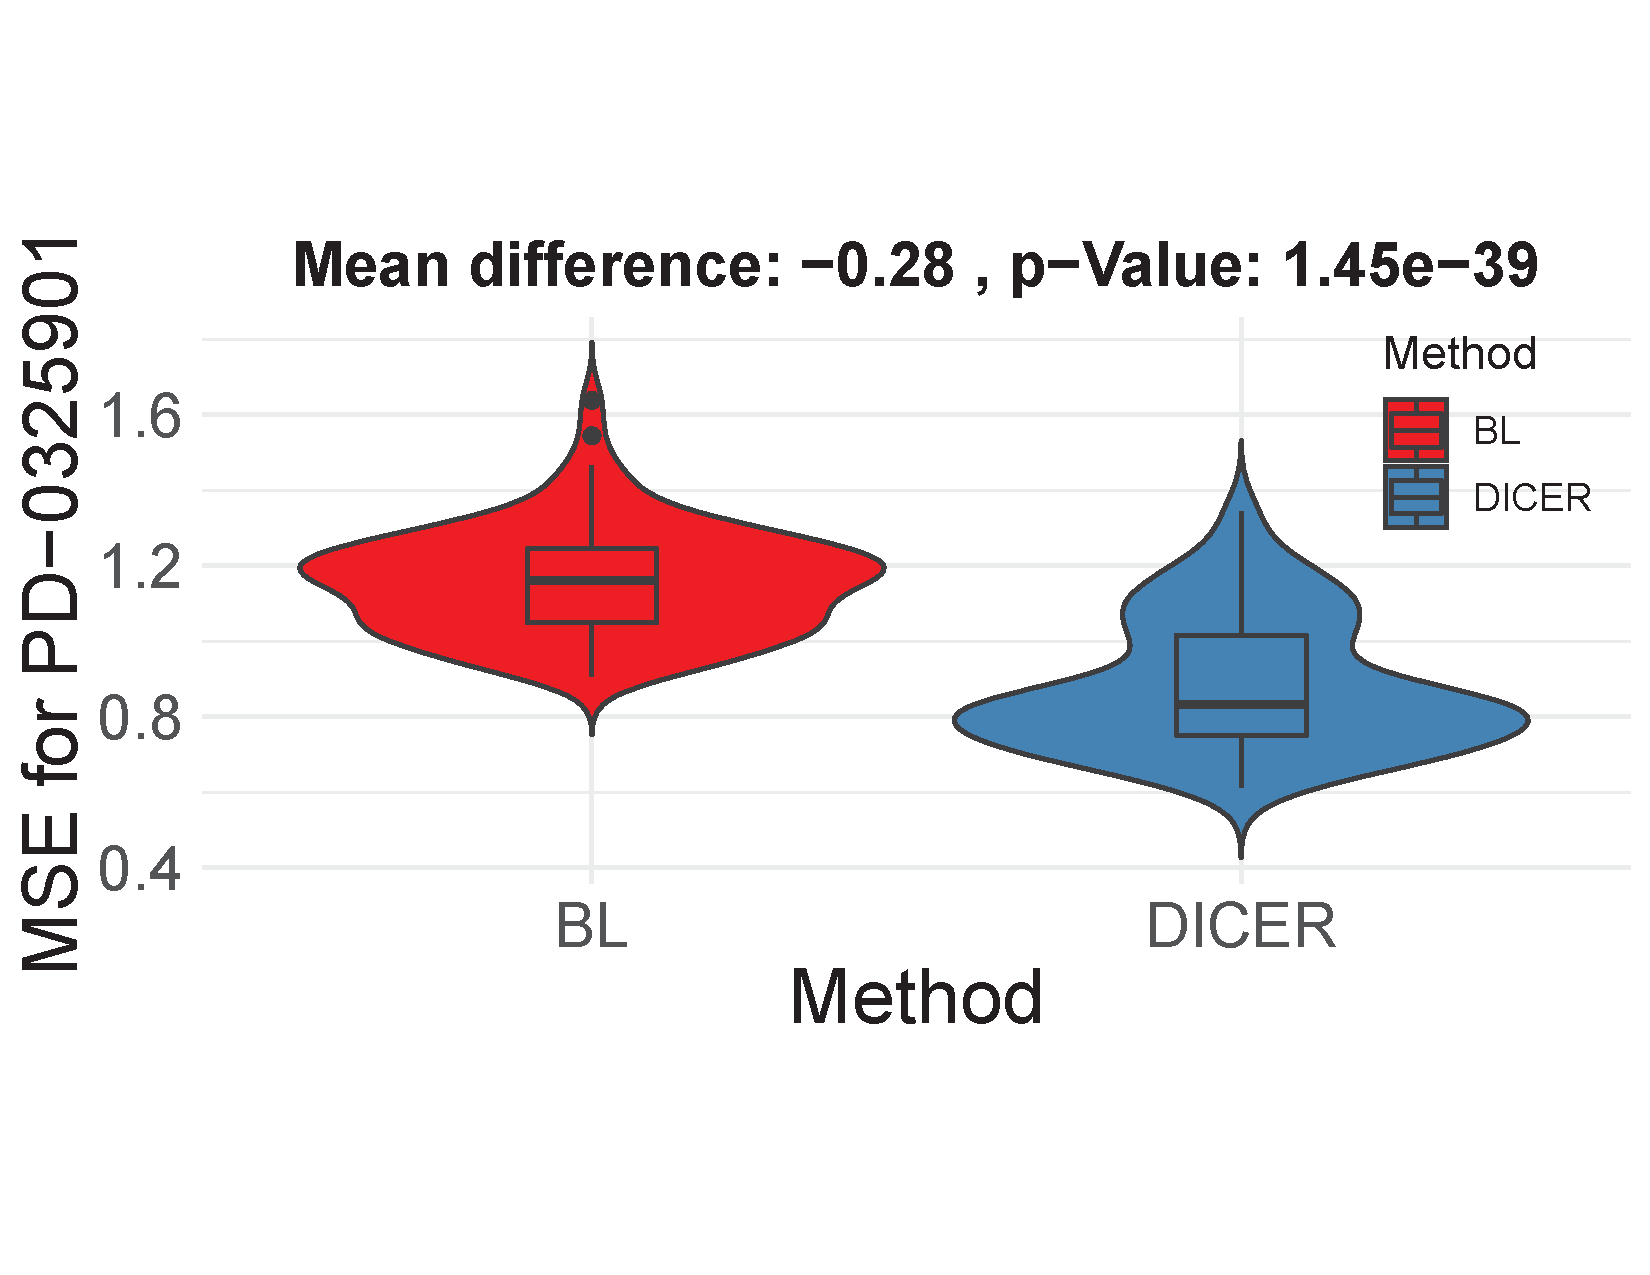
\includegraphics[width=\textwidth]{./img/bar1.pdf}
		\caption{}    
%		\label{fig:mean and std of net14}
	\end{subfigure}
	\hfill
	\begin{subfigure}[b]{0.22\textwidth}  
		\centering 
		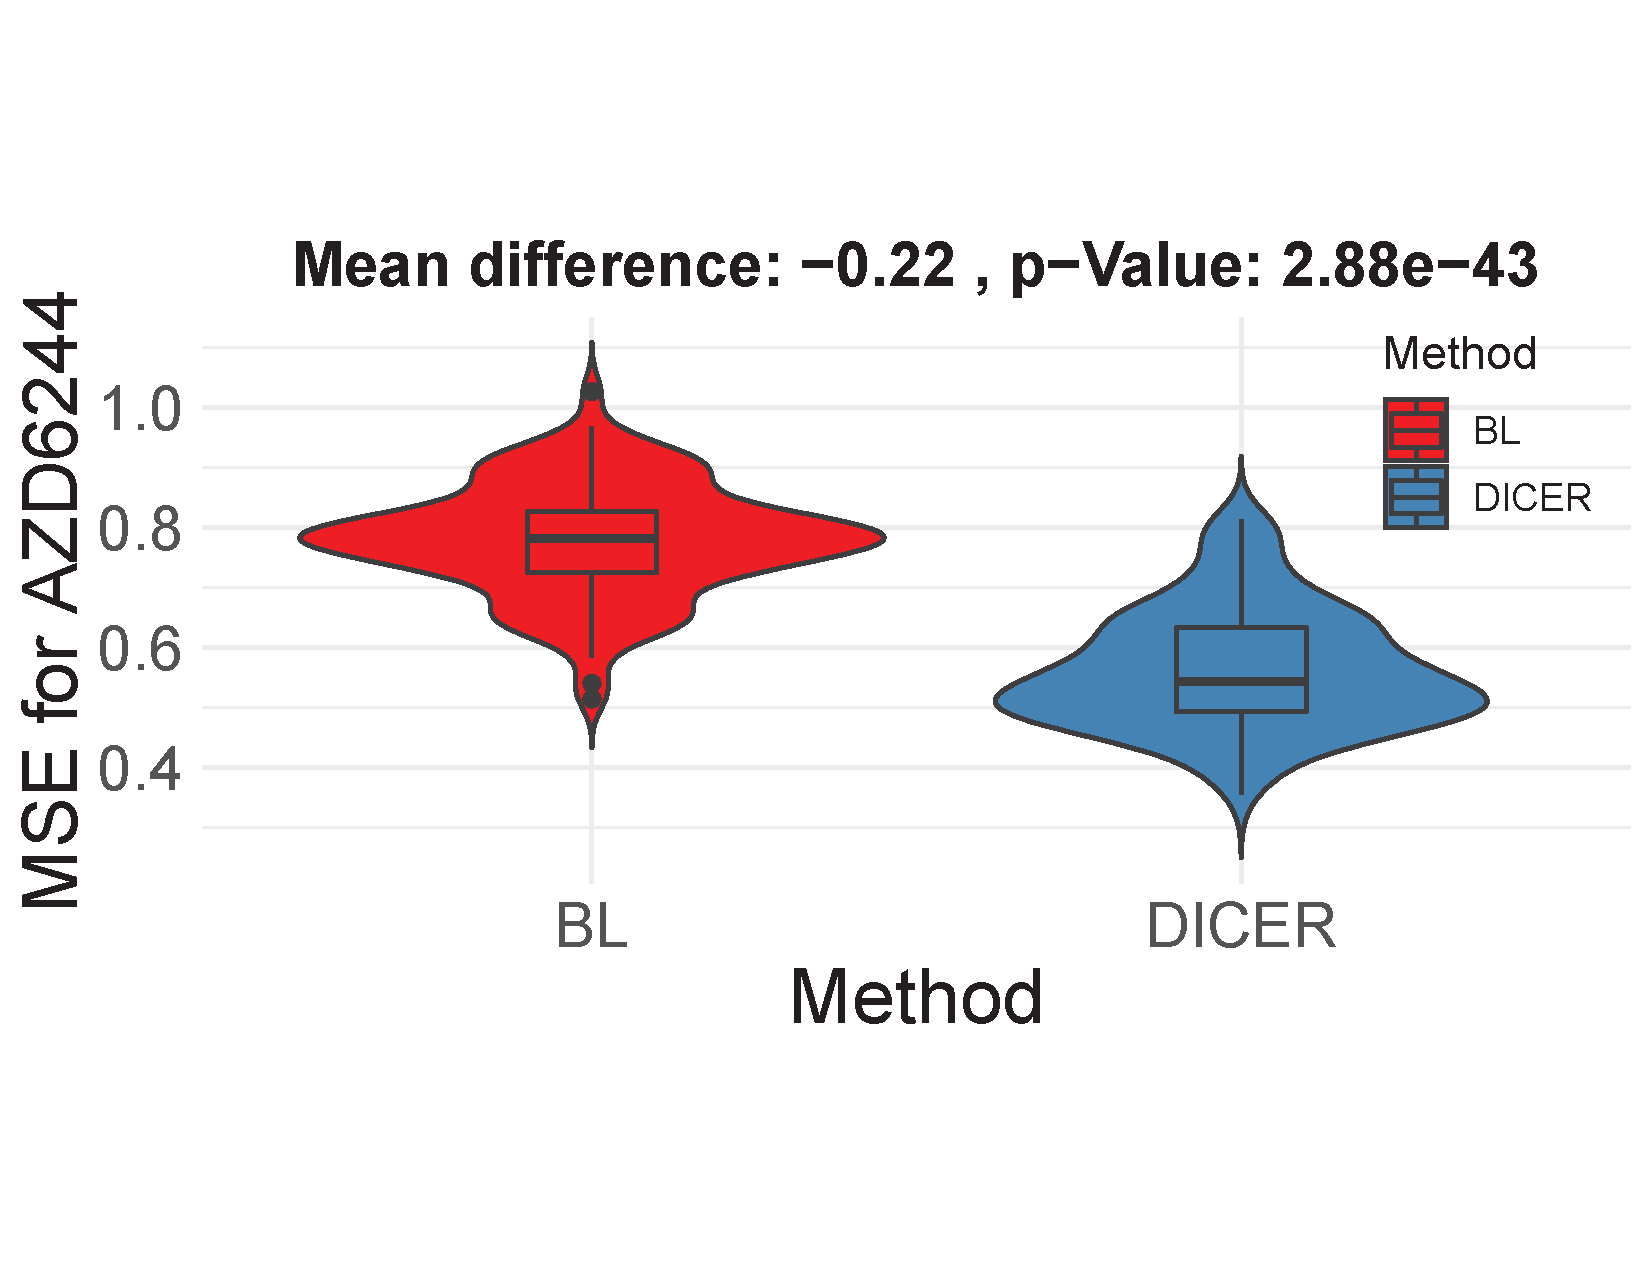
\includegraphics[width=\textwidth]{./img/bar2.pdf}
		\caption{}    
%		\label{fig:mean and std of net14}
	\end{subfigure}
	\vskip\baselineskip
	\begin{subfigure}[b]{0.22\textwidth}   
		\centering 
		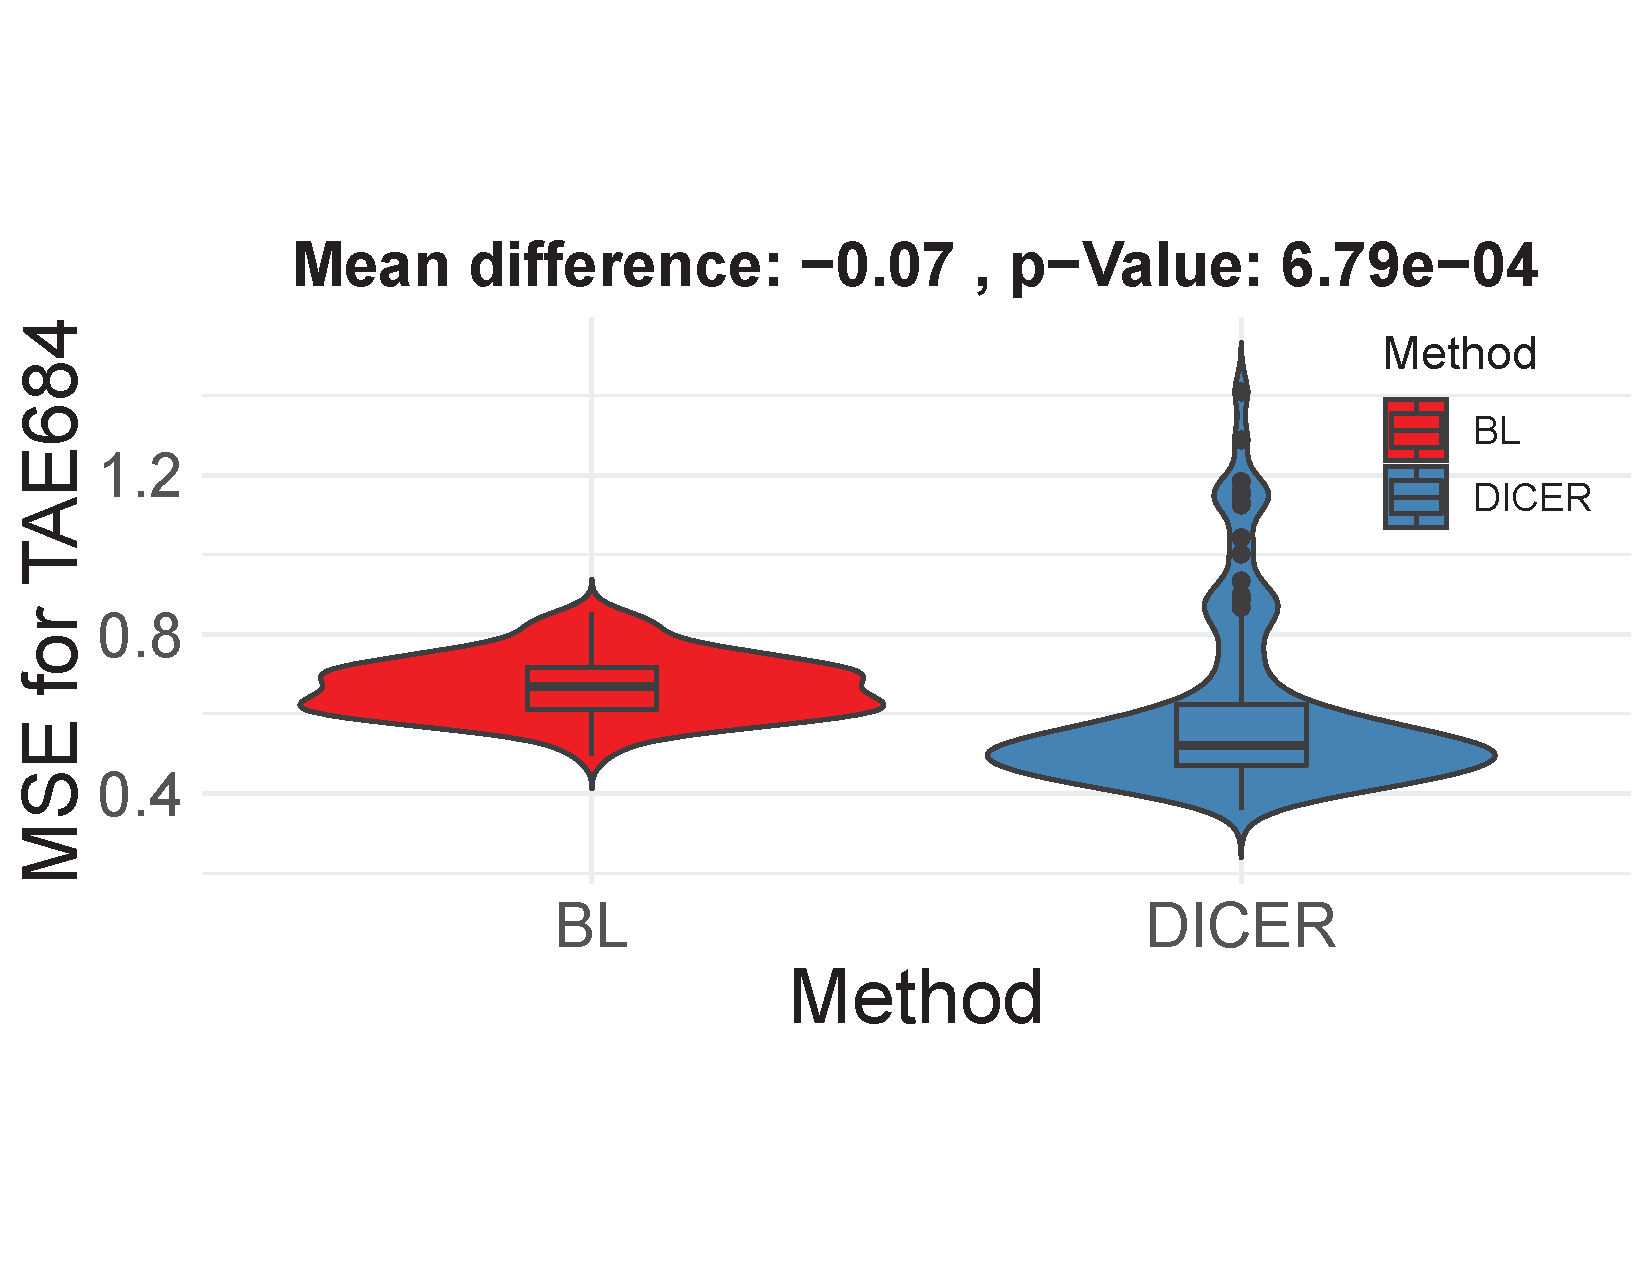
\includegraphics[width=\textwidth]{./img/bar3.pdf}
		\caption{}    
%		\label{fig:mean and std of net14}
	\end{subfigure}
	\quad
	\begin{subfigure}[b]{0.22\textwidth}   
		\centering 
		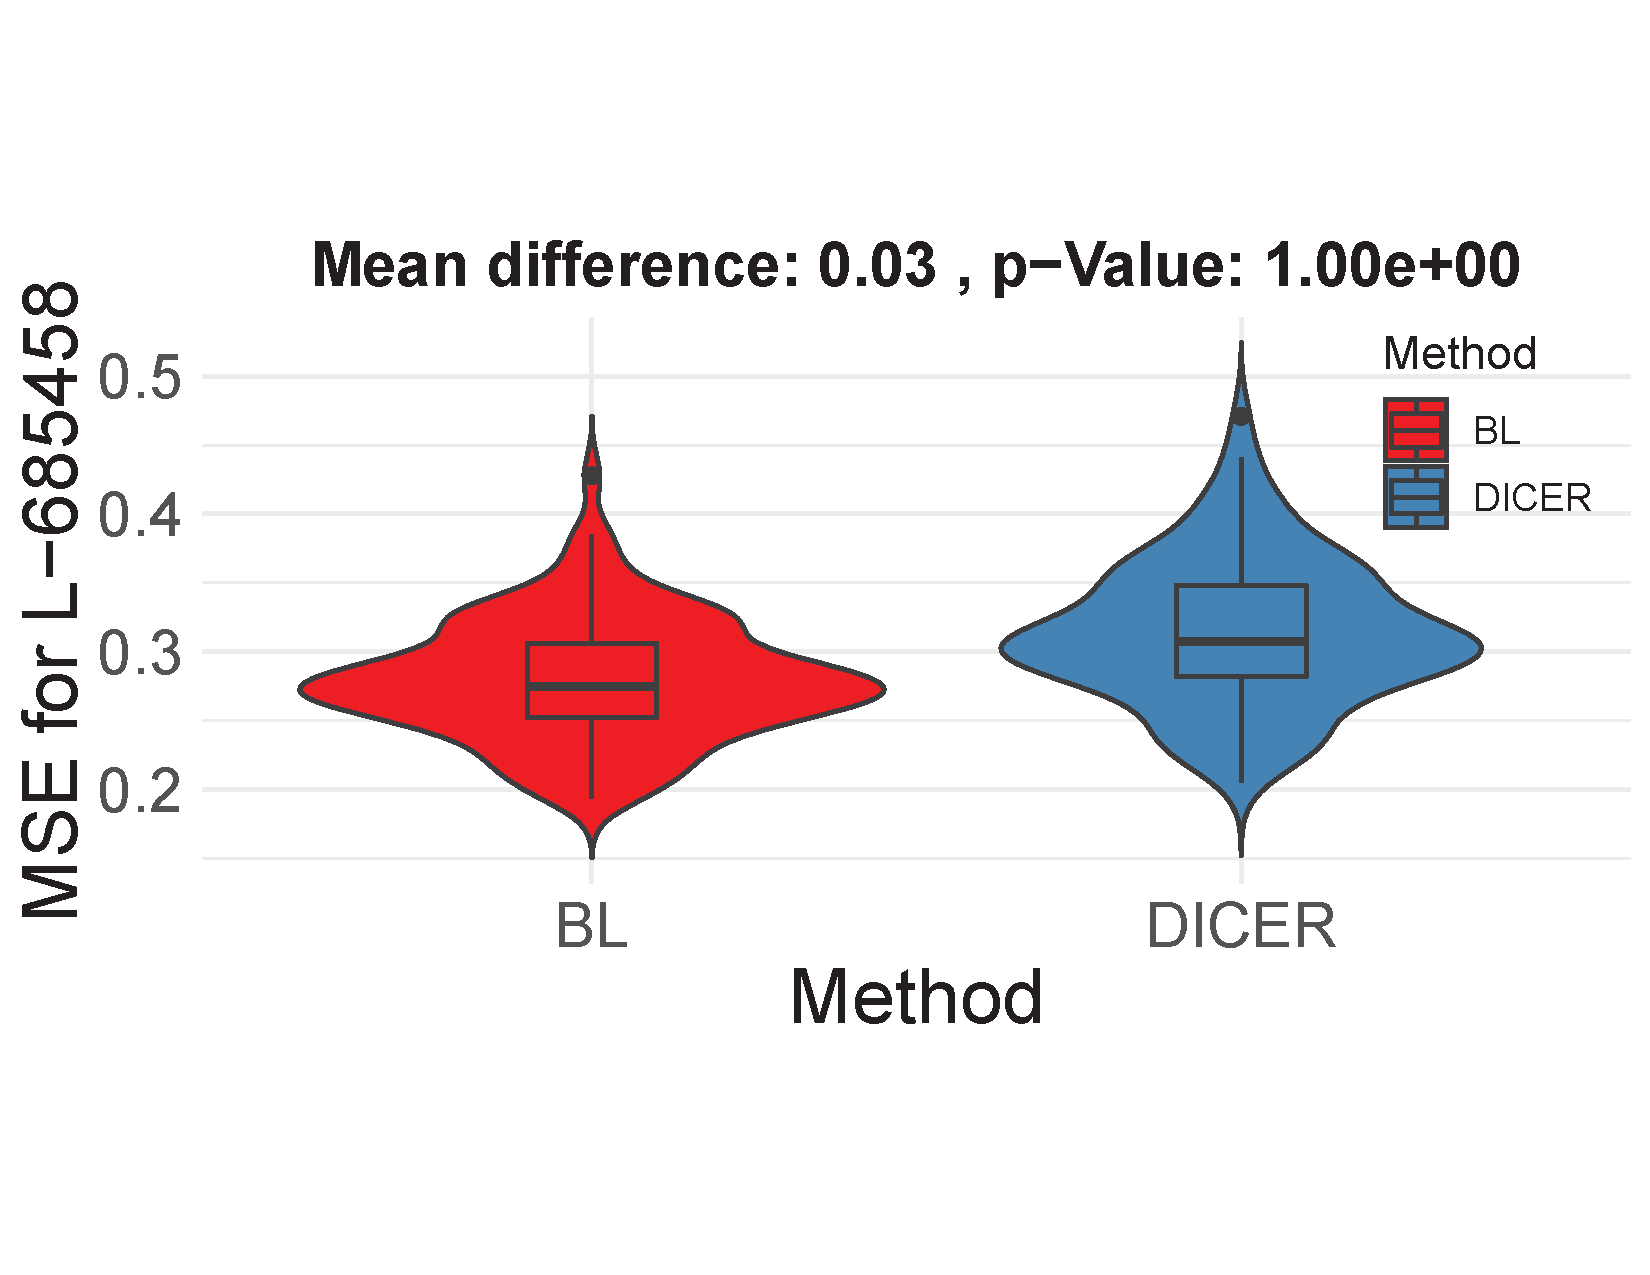
\includegraphics[width=\textwidth]{./img/bar4.pdf}
		\caption{}    
%		\label{fig:mean and std of net14}
	\end{subfigure}
	\squeezeup
	\caption{MSE for 100 bootstrapped dataset of four drugs of experiment TWO. (a),(b) Sample result of large difference between mean of MSEs and small p-values. (c) Smaller mean difference with significant p-value. (d) One of the three cases where \dc{} is outperformed by the baseline.} 
	\label{fig:allbars}
	\end{figure}


{\bf Interpretation}
%Next we focus on the interpretation of the selected genes. 
We select Saracatinib, a drug which shows activity on both lung and blood cancer cell lines, Figure \ref{fig:Saracatinib}. 
Then, during the bootstrap experiment of TWO, we record support of the estimated parameters by \dc. 
%Fixing the $d_g$ parameters, 
We pick the top five most frequently selected genes across 100 bootstrapped runs for further analysis. 
Now, we have three lists of genes for common, lung , and blood parameters. 
We perform gene enrichment analysis using ToppGene \cite{chen09toppgene} to see where in functional/disease/drug databases these genes have been observed together with statistical significance. 
Table \ref{table:1} summarizes a highlight of our findings which shows lung and blood parameters are correctly capturing a meaningful set of genes.% while the shared parameter has mixed set of genes. 
%{\small 
%\begin{tabular}{ |c|c|c|c|c|c|  }
%	\hline 	
%	\multicolumn{2}{|c|}{(Blood, 512)} & \multicolumn{2}{c|}{(Lung, 500)} & \multicolumn{2}{c|}{(Shared, 525)}\\
%	\hline
%	Highlights &    p-Val  & Highlights &    p-Val &  Highlights &    p-Val \\
%	\hline
%	regulation of immune response	 & 2.1E-8  & Secondary malignant neoplasm of lung & 8.9E-6  &  Acute	Myeloid Leukemia & 5.0E-7 \\
%	T cell activation	 & 5.0E-8   & Lung Cancer  & 2.9E-5  &  Chronic Myeloid Leukemia & 3.0E-5 \\
%	leukocyte activation & 1.0E-6  & Adenosquamous cell lung cancer	 & 3.9E-5  &  Adenocarcinoma of lung & 4.8E-5 \\
%	\hline
%\end{tabular}
%}
\begin{table*}
	\centering
	\begin{tabular}{ |c|c|c|c|  }
		\hline 	
		\multicolumn{2}{|c|}{(Blood, 512)} & \multicolumn{2}{c|}{(Lung, 500)}\\
		\hline
		Highlights &    p-Val  & Highlights &    p-Val   \\
		\hline
		Regulation of immune response	 & 2.1E-8  & Secondary malignant neoplasm of Lung & 8.9E-6  \\
		T cell activation	 & 5.0E-8   & Lung cancer  & 2.9E-5   \\
		Leukocyte activation & 1.0E-6  & Adenosquamous cell lung cancer	 & 3.9E-5 \\
		\hline
	\end{tabular}
\caption{Each column is (Cancer Type, Number of significant genes) and highlights show where the set of genes have been observed together. p-Values are computed by  Fisher's exact test \cite{chen09toppgene}.}
\label{table:1}
\end{table*}

%{ (Type, $|\text{supp}(\cdot)|$)} 	&   , ; 2.907E-5  & asd;flkajsdf ;as  &  asdf'alsdkfad' \\
%&   , stage IV;   & asd;flkajsdf ;as  &  asdf'alsdkfad' \\